\PassOptionsToPackage{unicode=true}{hyperref} % options for packages loaded elsewhere
\PassOptionsToPackage{hyphens}{url}
%
\documentclass[a4paperpaper,]{article}
\usepackage{lmodern}
\usepackage{amssymb,amsmath}
\usepackage{ifxetex,ifluatex}
\usepackage{fixltx2e} % provides \textsubscript
\ifnum 0\ifxetex 1\fi\ifluatex 1\fi=0 % if pdftex
  \usepackage[T1]{fontenc}
  \usepackage[utf8]{inputenc}
  \usepackage{textcomp} % provides euro and other symbols
\else % if luatex or xelatex
  \usepackage{unicode-math}
  \defaultfontfeatures{Ligatures=TeX,Scale=MatchLowercase}
\fi
% use upquote if available, for straight quotes in verbatim environments
\IfFileExists{upquote.sty}{\usepackage{upquote}}{}
% use microtype if available
\IfFileExists{microtype.sty}{%
\usepackage[]{microtype}
\UseMicrotypeSet[protrusion]{basicmath} % disable protrusion for tt fonts
}{}
\IfFileExists{parskip.sty}{%
\usepackage{parskip}
}{% else
\setlength{\parindent}{0pt}
\setlength{\parskip}{6pt plus 2pt minus 1pt}
}
\usepackage{hyperref}
\hypersetup{
            pdftitle={Moderate disturbances accelerate forest transition dynamics under climate change},
            pdfborder={0 0 0},
            breaklinks=true}
\urlstyle{same}  % don't use monospace font for urls
\usepackage[margin=1in]{geometry}
\usepackage{longtable,booktabs}
% Fix footnotes in tables (requires footnote package)
\IfFileExists{footnote.sty}{\usepackage{footnote}\makesavenoteenv{longtable}}{}
\usepackage{graphicx,grffile}
\makeatletter
\def\maxwidth{\ifdim\Gin@nat@width>\linewidth\linewidth\else\Gin@nat@width\fi}
\def\maxheight{\ifdim\Gin@nat@height>\textheight\textheight\else\Gin@nat@height\fi}
\makeatother
% Scale images if necessary, so that they will not overflow the page
% margins by default, and it is still possible to overwrite the defaults
% using explicit options in \includegraphics[width, height, ...]{}
\setkeys{Gin}{width=\maxwidth,height=\maxheight,keepaspectratio}
\setlength{\emergencystretch}{3em}  % prevent overfull lines
\providecommand{\tightlist}{%
  \setlength{\itemsep}{0pt}\setlength{\parskip}{0pt}}
\setcounter{secnumdepth}{0}
% Redefines (sub)paragraphs to behave more like sections
\ifx\paragraph\undefined\else
\let\oldparagraph\paragraph
\renewcommand{\paragraph}[1]{\oldparagraph{#1}\mbox{}}
\fi
\ifx\subparagraph\undefined\else
\let\oldsubparagraph\subparagraph
\renewcommand{\subparagraph}[1]{\oldsubparagraph{#1}\mbox{}}
\fi

% set default figure placement to htbp
\makeatletter
\def\fps@figure{htbp}
\makeatother

\usepackage{setspace}
\setstretch{1,5}
\usepackage{lineno}
\linenumbers

\title{Moderate disturbances accelerate forest transition dynamics under
climate change}
\date{}

\begin{document}
\maketitle

\hypertarget{list-of-authors}{%
\subsection*{List of authors}\label{list-of-authors}}
\addcontentsline{toc}{subsection}{List of authors}

Marie-Hélène Brice \textsuperscript{1,2} Steve Vissault
\textsuperscript{2,3} Willian Vieira \textsuperscript{2,3} Dominique
Gravel \textsuperscript{2,3} Pierre Legendre \textsuperscript{1,2}
Marie-Josée Fortin \textsuperscript{4}

\hypertarget{institutional-affiliations}{%
\subsection*{Institutional
affiliations}\label{institutional-affiliations}}
\addcontentsline{toc}{subsection}{Institutional affiliations}

\begin{enumerate}
\def\labelenumi{\arabic{enumi}.}
\tightlist
\item
  Département de Sciences Biologiques, Université de Montréal, Montréal,
  Québec, Canada.
\item
  Québec Centre for Biodiversity Sciences, McGill University, Montréal,
  Québec, Canada.
\item
  Département de biologie, Université de Sherbrooke, Sherbrooke, Québec,
  Canada.
\item
  Department of Ecology and Evolutionary Biology, University of Toronto,
  Toronto, Ontario, Canada.
\end{enumerate}

\hypertarget{contact-information}{%
\subsection*{Contact Information}\label{contact-information}}
\addcontentsline{toc}{subsection}{Contact Information}

Marie-Hélène Brice

\begin{itemize}
\tightlist
\item
  email: marie-helene.brice@umontreal.ca
\end{itemize}

\hypertarget{running-title}{%
\subsection{Running title}\label{running-title}}

?

\hypertarget{abstract-draft}{%
\section{Abstract {[}draft{]}}\label{abstract-draft}}

Several temperate tree species in North America are expected to expand
their distribution northward, where the boreal forest is already
established and dominated by conifers. However, these transitions from
boreal to mixed and from mixed to temperate forests could be hampered by
non-climatic factors, such as unsuitable soil conditions and competition
by resident species.

In this paper, we describe the state transition dynamics of Quebec's
forest communities in recent decades and identify the factors and
processes that promote or prevent these state transitions. Specifically,
we ask (1) Is forest transition dynamic affected by recent climate
change? (2) How do disturbances and soil characteristics influence the
transition probability among forest states under climate change? Can
natural or anthropogenic disturbances accelerate climate related
transitions? And, conversely, can soil characteristics constrain these
transitions? (3) How do different disturbance type and intensity
influence the transient dynamics and equilibrium distribution of forest
states?

To answer these questions, we analyzed the transition dynamics in over
10,000 forest inventory plots of southern Quebec (1970-2016). Using a
continuous time Markov multi-state model, we investigated the
relationship between the transition probabilities between the different
states of the forest community (temperate, boreal, mixed and pioneer)
and variables related to climate, local soil conditions and
disturbances. We also describe the long-term equilibrium state
distribution under different disturbance scenarios, as well as the
transient dynamics using complementary measures: the time to reach
equilibrium, the turnover time and the entropy of the modeled system.

The transition probabilities are mainly related by natural and
anthropogenic disturbances and secondarily to climatic variables,
whereas soil characteristics (drainage and pH) were not a strong
constraint. Moreover, moderate disturbances increased the probability of
transition from Mixed to Temperate forests and thus accelerate long-term
climate-induced transitions. {[}equilibrium\ldots{} transient
dynamic\ldots{}{]}

Moderate disturbances were found to catalyze rapid transitions in forest
communities and accelerate shift in response to recent climate change.
In ecotones, areas of ecological tension, disturbances may provide
opportunities for some migrating species to establish in otherwise
competitive environments\ldots{}

\hypertarget{keywords}{%
\subsection{Keywords}\label{keywords}}

Climate change, Disturbances, Forest, Continuous-time Markov model,
Multi-state model, Québec, Temperate-boreal ecotone, Transition
probabilities, Resilience

\pagebreak

\hypertarget{introduction}{%
\section{Introduction}\label{introduction}}

\hypertarget{p1.-forest-dynamics-under-cc}{%
\subsection{\texorpdfstring{\emph{P1. Forest dynamics under
CC}}{P1. Forest dynamics under CC}}\label{p1.-forest-dynamics-under-cc}}

Global climate warming is forcing species to move (Parmesan \& Yohe,
2003). In the temperate-boreal forest ecotone, several temperate
deciduous tree species are slowly migrating northward, colonizing
conifer dominated forests (Boisvert-Marsh, Périé, \& de Blois, 2014;
Evans \& Brown, 2017; Fisichelli, Frelich, \& Reich, 2014; Sittaro,
Paquette, Messier, \& Nock, 2017). As climate warms and tips the balance
in favor of temperate over boreal species, forests may transition from
coniferous to mixedwood and from mixedwood to temperate deciduous
(Boulanger et al., 2019; Price et al., 2013). While boreal forest
dynamic is characterized by broad-scale disturbances, mainly fires and
insect outbreaks, and slow decomposition of an acidic and nutrient poor
litter, temperate forest dynamic is characterized by small scale canopy
gaps and rapid decomposition of a rich litter (Goldblum \& Rigg, 2010).
Hence, as ecological processes strongly differ among those biomes,
climate-induced range shifts not only impact species distributions, but
also alter the structure of communities, microclimates, biogeochemical
cycles and ecosystem functioning and thus trigger a ``regime shift''
(Scheffer, Carpenter, Foley, Folke, \& Walker, 2001).

While tree climate niches are expected to shift northward by several
hundred kilometers by the end of the century (McKenney, Pedlar,
Lawrence, Campbell, \& Hutchinson, 2007), multiple studies indicate that
tree migration will not keep pace with global warming (e.g.~ Zhu,
Woodall, \& Clark, 2012; Renwick \& Rocca, 2015; Sittaro et al., 2017;
Talluto, Boulangeat, Vissault, Thuiller, \& Gravel, 2017; Vissault,
2016; Woodall et al., 2013). The slow response of forests to
environmental changes is not surprising given that trees cannot walk,
live for several decades to centuries and disperse over very short
distance. Hence, if forests are undisturbed, the speed of transitions
between forest biomes will be mainly limited by the natural turnover
rate of the resident species as well as the dispersal and establishment
rates of the migrating species (Neilson, 1993). However, as the
disequilibrium between climate conditions and forest composition grows
larger, alternative stable states become possible and forests may fail
to return to their previous state following a disturbance (Johnstone et
al., 2016).

\hypertarget{p2.-disturbances}{%
\subsection{\texorpdfstring{\emph{P2.
Disturbances}}{P2. Disturbances}}\label{p2.-disturbances}}

Both gradual and abrupt transitions from one biome to another will
likely take place concurrently, but, as forests are increasingly
subjected to both pervasive climatic stresses and direct human-related
disturbances, catastrophic transitions are likely to play a dominant
role in driving the climate shift in biomes. Established communities are
generally though to be resistant to competitive displacement and
resilient to commonly experienced disturbances (Grondin et al., 2018;
Seidl, Rammer, \& Spies, 2014). Resistance can be defined as the ability
of an ecosystem to persist through time following a disturbance, whereas
resilience is the capacity to recover its pre-disturbance composition
(Gunderson, 2000; Holling, 1973). Because the ability to persist and
recover following a pulse disturbance (e.g., fire or logging) can be
altered by a press disturbance (e.g., climate change), investigating
resistance and resilience can provide precious insights into their
interacting effects.

However, as climate change weaken forest resilience, disturbances can
provide niche opportunities for migrating species and community
composition can shift abruptly to species that are better suited to
current conditions (Johnstone et al., 2016; Renwick \& Rocca, 2015;
Turner, 2010). For example, canopy gaps have been shown to locally
facilitate establishment of temperate species in mixed forests of
Ontario (Leithead, Anand, \& Silva, 2010). In Alaska, white spruce
(\emph{Picea glauca}) is invading black spruce (\emph{Picea mariana})
stands following fire and permafrost degradation (Wirth, Lichstein,
Dushoff, Chen, \& Chapin, 2008). Similarly, moderate disturbances
favored the increase of warm-adapted species and led to a broad-scale
community thermophilization of forests in Québec (Brice, Cazelles,
Legendre, \& Fortin, 2019). However, the coupling of warming and
disturbances may depend on the intensity and type (natural or
anthropogenic) of disturbances (Johnstone, Hollingsworth, Chapin, \&
Mack, 2010). Hence, in some cases, disturbances can promote invasions by
early successional species which then displace long-lived
shade-tolerant. For instance, clearcutting has been found to favor the
expansion of trembling aspen (\emph{Populus tremuloides}) in mixed and
boreal stands of Québec (Grondin et al., 2018; Laquerre, Leduc, \&
Harvey, 2009) and Alberta (Landhäusser, Deshaies, \& Lieffers, 2010). In
contrast, other simulation studies have found that, although
disturbances can influence some types of transitions, they are unlikely
to drive extensive biome shifts in the coming decades (Liang, Duveneck,
Gustafson, Serra-Diaz, \& Thompson, 2018; Vanderwel \& Purves, 2014). As
a result, disturbances could accelerate shifts to an increasingly
deciduous‐dominated landscape, but empirical evidence of this process
are necessary to understand how various intensities and types of
disturbances may catalyze or hinder transitions between certain forest
states.

\emph{other ref: Xu, Gertner, \& Scheller (2012); Danneyrolles et al.
(2019); Johnstone \& Chapin (2003)}

\hypertarget{p3.-soil}{%
\subsection{\texorpdfstring{\emph{P3. Soil}}{P3. Soil}}\label{p3.-soil}}

The northward migration of temperate species might be further
constrained by their capacity to colonize different types of soil
(Bennett et al., 2017; Brown \& Vellend, 2014; Lafleur, Paré, Munson, \&
Bergeron, 2010). Indeed, soils of cold boreal forests generally have
lower pH, lower microbial activity and slower decomposition rate of
organic matter than warmer southern temperate forests (Goldblum \& Rigg,
2010). These local and regional variations in soil properties (e.g.,
quality of drainage, availability of nutrients, pH, mycorrhizae) are
expected to slow down or inhibit the establishment of temperate trees
into the boreal forest. For instance, transplant experimental studies
have shown that seedlings of sugar maple (\emph{Acer saccharum}) in
conifer-dominated stands were negatively affected by seed predators and
fungal pathogens (Brown \& Vellend, 2014) as well as by soil acidity
through reduced foliar nutrition (Collin, Messier, \& Bélanger, 2017).
However, Kellman (2004) found that, after initial high mortality due to
seed predation, survival of \emph{Acer saccharum} seedling in boreal
stands was high, even superior to that in the temperate stands,
potentially because of increased light availability. Hence, it has been
suggested that soil properties in boreal forests may not be a major
impediment to the migration of temperate species showing broad
ecological tolerance (Barras \& Kellman, 1998; Kellman, 2004; Lafleur et
al., 2010). Nonetheless, suboptimal soil conditions could delay forest
transition under climate change (Brown \& Vellend, 2014) and, moreover,
waterlogged conditions and deep organic matter accumulation may prevent
the regeneration of several species (Lafleur et al., 2010). While
experimental studies provide valuable insights on the potential role of
soils at local scales, we need to test the generality of such
constraints, or the lack thereof, on long term forest dynamic, across
species and across scales to better anticipate future biome transition.

\hypertarget{p4.-markov-multi-state-models}{%
\subsection{\texorpdfstring{\emph{P4. Markov multi-state
models}}{P4. Markov multi-state models}}\label{p4.-markov-multi-state-models}}

One approach to investigating the process of biome shifts in response to
climate change is to model transition probabilities of forest plots
among states based upon the knowledge of their current state, as well as
their current environmental characteristics. Given the unequivocal
distinction between temperate and boreal forests, the dynamic of tree
communities at ecotone can be adequately characterized using discrete
functional and successional states, namely Boreal, Mixed, Temperate and
Pioneer (Vissault, 2016) and thus can be formalized as a multi-state
Markov model (Jackson, 2018). Markov models provide a useful framework
for modeling changes of state over time using longitudinal data. In
epidemiology, for example, the models are often used to describe the
progression of diseases (Van Den Hout, 2016). In ecology, the models
have been used to study processes such as ecological succession (Hill,
Witman, \& Caswell, 2004; Runkle, 1981), metapopulation dynamics (Hanski
\& Ovaskainen, 2003; Moilanen, 1999), landcover changes (Muller \&
Middleton, 1994; Yang, Zheng, \& Chen, 2014), or stage class transitions
(Caswell, 2008).

Despite the simplicity of a four-state transition model, this modeling
framework allows to answer questions related to the coarse-scale
dynamics of biome shift. Moreover, without explicitly modeling them,
multi-state models represent mechanisms (Wootton, 2001). For example,
transitions to pioneer reflect disturbance, transitions from pioneer
reflect colonization, dispersal and recruitment limitation and
transitions between the other states reflect competition. In addition to
their simplicity, there exists numerous well‐established properties of
Markov transition matrices (Hill et al., 2004). Transition matrices can
be estimated from the model output and their properties can then be
compared under different scenarios to further explore the mechanisms of
forest dynamics. For instance, the steady state distribution can be
derived from a transition matrix and allow to infer the long-term forest
composition {[}REF{]}. Multi-state models can not only be used to
explicitly test hypotheses about equilibrium, but they can also be used
to describe state changes during dynamic periods, i.e.~transient
dynamics (Boulangeat, Svenning, Daufresne, Leblond, \& Gravel, 2018). As
most ecosystems never reach equilibrium (Holling, 1973), transient
dynamics, especially in forests, may persist over very long time periods
and are now thus recognized as crucial part of ecosystem dynamics
{[}REF{]}. The time of convergence to reach the steady state
distribution describes how fast the system converges; the turnover time
indicates how fast the transitions occur and provides insights about the
stability and the resistance of a forest state, while the entropy
reveals the predictability of the transitions. Contrasting empirically
derived transition matrices and their properties among disturbance
scenarios can shed new light on forest dynamics under climate change and
may even provide insights on management measures.

\hypertarget{p5.-objectives}{%
\subsection{\texorpdfstring{\emph{P5.
Objectives}}{P5. Objectives}}\label{p5.-objectives}}

In this paper, we investigate the response of forests to recent climate
warming by estimating the transition probability among four community
states, boreal, mixed, temperate and pioneer. Specifically, we address
these questions: 1. Is forest transition dynamic affected by recent
climate change? 2. How do disturbances and soil characteristics
influence the transition probability among forest states under climate
change? Can natural or anthropogenic disturbances catalyze climate
related transitions? And, conversely, can soil characteristics constrain
these transitions? 3. How do different disturbance type and intensity
influence the transient dynamics and equilibrium distribution of forest
states?

We expect that the probability of self transitions will be the highest,
i.e. most forests will not change states, because of tree slow
demography. However, climate warming should promote more transitions
from boreal to mixed forests and from mixed to temperate than the
reverse. We also anticipate that natural and anthropogenic disturbances
will further favor these climate-related transitions while soil
characteristics will slow them down. We apply a time-continuous
multi-state model to the dynamics of forest communities to estimate
state transition probabilities and evaluate the influence of
environmental covariates on these transitions. Using the result from our
multi-state model, we investigate the impact of disturbances on forest
equilibrium and transient dynamics under recent climate change using
several measures: equilibrium state distribution, time to converge to
equilibrium, turnover time and entropy.

\hypertarget{methods}{%
\section{Methods}\label{methods}}

\hypertarget{study-area-and-forest-inventory-data}{%
\subsection{Study area and forest inventory
data}\label{study-area-and-forest-inventory-data}}

To investigate large-scale transition dynamics in forest communities, we
used forest inventory plots in Quebec, Canada, which have been sampled
approximately every ten years since 1970 and ongoing by the Ministère
des forêts, de la Faune et des Parcs (MFFP, 2016). The study area
extends from approximately 45° to 52°N of latitude (ca. 795 000
km\textsuperscript{2}) and covers six bioclimatic domains and three
different forest subzones (Fig. 1). The mixed forest (from 47°N to 48°N)
marks the transition between the hardwood forest to the south, which is
dominated by \emph{Acer saccharum}, and the boreal forest to the north,
which is dominated by \emph{Abies balsamea} and \emph{Picea mariana}.

We selected all inventory plots that were sampled at least twice as well
as the ones where soil covariates were available. We disregarded plots
that were subjected to active reforestation during the study period
because we were interested in transition dynamics resulting from natural
recolonization. This yielded a total of 10,388 plots analyzed (Fig. 1).
The time intervals between plot surveys varied from 4 to 43 years, with
a mean time of 11 years (\(\sigma\) = 3.85).

\begin{figure}
\centering
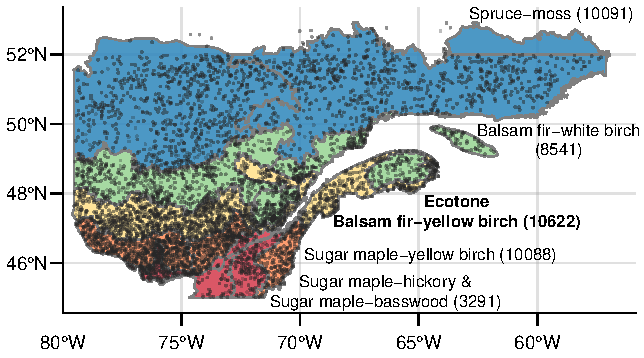
\includegraphics{res/fig1_region.pdf}
\caption{Locations of the 10,388 forest inventory plots in meridional
Québec, Canada. Colors delimit the six bioclimatic domains. The two
southernmost domains (red) are here combined. The number of forest plots
in each domain is written in parentheses. The balsam fir-yellow birch
domain is the ecotonal zone between hardwood and boreal forests.}
\end{figure}

\hypertarget{community-states}{%
\subsection{Community states}\label{community-states}}

We classified the forest inventory plots into four community states
(Boreal, Mixed, Temperate and Pioneer) using species basal area and
composition at each sampling date. We first assigned each studied
species as boreal, temperate or pioneer according to their functional
traits (see Table SX in Brice et al., 2019). For each plot, we computed
the total basal area of each species group and then classified the plot
following the MFFP (2016) definitions to one of the four states; Boreal
(boreal species represent \textgreater{}75\% of the plot basal area),
Temperate (temperate species represent \textgreater{}75\% of the plot
basal area), Mixed (temperate and boreal species both occupy between
\textgreater{}25\% and \textless{}75\% of the plot basal area) and
Pioneer (pioneer species represent \textgreater{}75\% of the plot basal
area or plot total basal area \textless{}5m\textsuperscript{2}/ha). We
analyzed state transitions between each consecutive plot survey. Based
on this classification, from the 38,091 observations (plots x number of
years measured), we observed 27,703 state transitions (Fig. 2).

\hypertarget{environmental-variables}{%
\subsection{Environmental variables}\label{environmental-variables}}

The annual past climatic conditions, covering a period from 1960 to
2013, were extracted from a 2km\textsuperscript{2} (60 arc sec)
resolution grid for the entire study area using the ANUSPLIN climate
modelling software (http://cfs.nrcan.gc.ca/projects/3/8; McKenney et
al., 2011). Plot locations were intercepted with two bioclimatic
variables hypothesized to influence tree establishment, survival and
growth: the mean temperature during the growing season and the annual
climate moisture index (CMI), which is the difference between annual
precipitation and potential evapotranspiration (Table 1). To reduce the
effect of inter-annual climate variability, each climate variable was
averaged over a 10-year period prior to the plot measurement. Over the
past four decades, growing season temperature have increased by 0.14
°C/decade, while CMI has decreased by 1.2 cm/decade.

We also collected information pertaining to natural and anthropogenic
disturbances that have affected the forest plots during the study period
(Table 1). At each plot, the type of disturbances (21 types) and their
level of intensity (moderate or major) were recorded (see Table S2 in
Brice et al., 2019; MFFP, 2016). The MFFP defined major disturbances as
events that have eliminated more than 75\% of the tree basal area,
whereas moderate disturbances have eliminated between 25\% and 75\%. For
our multi-state model, we differentiated two main types of disturbances:
natural disturbances and harvest, with three levels of intensity each
(minor, moderate or major).

Finally, at each plot, several edaphic characteristics were recorded
(MFFP, 2016). Of the available variables, we selected drainage and pH
because they largely affects nutrient availability, soil structural
properties and vegetation development {[}REF{]}. These two variables
also capture most of the variance in soil characteristics in plots
across Quebec and were orthogonal in a PCA (not shown).

Table 1. Description of the covariates used in the multi-state models.

\begin{longtable}[]{@{}ll@{}}
\toprule
\begin{minipage}[b]{0.21\columnwidth}\raggedright
Covariate name\strut
\end{minipage} & \begin{minipage}[b]{0.73\columnwidth}\raggedright
Covariate description\strut
\end{minipage}\tabularnewline
\midrule
\endhead
\begin{minipage}[t]{0.21\columnwidth}\raggedright
\textbf{Climate}\strut
\end{minipage} & \begin{minipage}[t]{0.73\columnwidth}\raggedright
\strut
\end{minipage}\tabularnewline
\begin{minipage}[t]{0.21\columnwidth}\raggedright
Temp\strut
\end{minipage} & \begin{minipage}[t]{0.73\columnwidth}\raggedright
Mean temperature during growing season, 10-year average prior to first
measurement (°C).\strut
\end{minipage}\tabularnewline
\begin{minipage}[t]{0.21\columnwidth}\raggedright
CMI\strut
\end{minipage} & \begin{minipage}[t]{0.73\columnwidth}\raggedright
Mean annual Climate Moisture Index, 10-year average prior to first
measurement (cm).\strut
\end{minipage}\tabularnewline
\begin{minipage}[t]{0.21\columnwidth}\raggedright
\textbf{Soil}\strut
\end{minipage} & \begin{minipage}[t]{0.73\columnwidth}\raggedright
\strut
\end{minipage}\tabularnewline
\begin{minipage}[t]{0.21\columnwidth}\raggedright
pH\strut
\end{minipage} & \begin{minipage}[t]{0.73\columnwidth}\raggedright
pH of of the surface horizon\strut
\end{minipage}\tabularnewline
\begin{minipage}[t]{0.21\columnwidth}\raggedright
Drainage\strut
\end{minipage} & \begin{minipage}[t]{0.73\columnwidth}\raggedright
7 classes of soil drainage, which range from excessive to very poor,
that were treated as numeric.\strut
\end{minipage}\tabularnewline
\begin{minipage}[t]{0.21\columnwidth}\raggedright
\textbf{Disturbances}\strut
\end{minipage} & \begin{minipage}[t]{0.73\columnwidth}\raggedright
\strut
\end{minipage}\tabularnewline
\begin{minipage}[t]{0.21\columnwidth}\raggedright
Logging\strut
\end{minipage} & \begin{minipage}[t]{0.73\columnwidth}\raggedright
Tree harvesting, including clearcutting, selection cutting, shelterwood
cutting, seed-tree cutting, etc. None or minor (0), moderate (1) or
major (2).\strut
\end{minipage}\tabularnewline
\begin{minipage}[t]{0.21\columnwidth}\raggedright
Natural\strut
\end{minipage} & \begin{minipage}[t]{0.73\columnwidth}\raggedright
Natural disturbances, including forest fires, insect outbreaks,
windfall, etc. None (0), moderate (1) or major (2).\strut
\end{minipage}\tabularnewline
\bottomrule
\end{longtable}

\hypertarget{analysis}{%
\subsection{Analysis}\label{analysis}}

\emph{NB: very detailed\ldots{} where can we cut?}

\emph{NB2: Lot of mathematical equations with different letters\ldots{}
verify if everything matches!}

\hypertarget{continuous-time-multi-state-markov-model}{%
\subsubsection{Continuous-time multi-state Markov
model}\label{continuous-time-multi-state-markov-model}}

We derived our modeling framework from methods widely used in survival
analysis and disease progression model (Jackson, 2018; Van Den Hout,
2016). Similarly to Vissault (2016), we formalized forest dynamics as a
four-state model, but here we used a continuous-time multi-state model
(Jackson, 2018) in which transitions among states depend on the previous
state, time interval, climate, disturbances and soil characteristics
(Fig. 2).

In ecology, Markov models are often built using discrete time steps.
However, because (1) time interval between surveys are irregular, (2)
for each time interval, multiple transitions are possible and (3) the
exact times of state changes are unobserved (i.e.~observations are
interval-censored), a continuous-time Markov model, in which time is
treated as continuous, is preferable. Given observations at fixed time
intervals, a homogeneous continuous-time Markov chain is a special case
of a discrete-time Markov chain.

For states \(r,s \in {B, M, P, T}\) and time \(h,t ≥ 0\), transition
probabilities (\(p_{rs}\)) are defined as the probability that a plot in
state \(r\) at time \(h\) is in state \(s\) at time \(h + t\) and can be
denoted by:

\(P_{r,s}(h, t) = P(S_{h+t} = s | S_{h} = r)\).

The Markov process is assumed to be time homogeneous, meaning that the
transition probabilities are constant over time (i.e.~independent of
\(t\), but dependent of the time interval), hence
\(P(S_{h+t} = s | S_{h} = r) = P(S_{t} = s | S_{0} = r)\). However, this
assumption can be relaxed (see below). In a four-state transition model,
the transition probability matrix \(P(t)\) is a 4 \(\times\) 4 matrix,
where the rows are the current state and the columns the future state,
containing the transition probabilities \(p_{rs}(t)\) for a specified
time interval. For a time-homogeneous model, \(P(t)\) can be solved by
taking the matrix exponential of the intensity or generator matrix \(Q\)
scaled by the time interval:

\(P(t) = e^{tQ}\)

The intensity matrix \(Q\) contains transition intensities \(q_{r,s}\)
which represent the instantaneous risk of moving from state \(r\) to
state \(s\):

\(q_{r,s} = \lim_{\Delta \to 0} \frac{P(Y_{t+\Delta} = s | Y_t = r)}{\Delta}\),
on off-diagonal elements.

\(q_{r,r} = − \sum_{s \neq r}{q_{rs}}\), on diagonal elements.

Transition-specific hazard regression models can be defined for those
\(r,s \in S\) between which a direct transition is possible according to
the specified multi-state process (Fig. 2). The intensities \(q_{r,s}\)
can be modeled as a combination of a baseline hazard \(q_{rs.0}\) with a
vector of explanatory variables \(x(t)\) and a vector of coefficients
\(\beta_{rs}\) :

\(q_{rs}(t) = q_{rs}(t|x(t)) = q_{rs.0}(t)exp(\beta_{rs}'x(t))\),

The definition of the log-linear regression hazard model allows to fit a
site-specific and time-dependent covariate vector \(x(t)\) to transition
intensities. Time-dependent covariates, such as climate and
disturbances, are assumed to be piecewise-constant, i.e.~the hazard is
constant within a specified time interval \([h, h+t]\) and depends on
the covariate value at \(h\), but is allowed to change between the
intervals. The time homogeneity assumption is thus relaxed by the
inclusion of time-dependent covariates in the model.

Estimation of model parameters can be obtained by maximizing the
log-likelihood function using the transition probability matrix. The
contribution of the plot \(i\) at time \(j\) to the likelihood is given
by:

\(LL_i(\theta | s,x) = \prod\limits_{j=1}^{J} P(S_j=s_j|S_{j-1}=s_{j-1},\theta,x)\),

where \(\theta\) is the vector with all the model parameters, \(x\)
denotes the vector with the covariate values, and \(s\) denotes the
observed state trajectory \(s_1,...,s_J\) at times \(t_1,...,t_J\). The
full likelihood function is the product of contributions for all \(N\)
plots:

\(LL(\theta) = \prod\limits_{i=1}^{N} LL_i(\theta | s,x)\),

\hypertarget{definition-of-candidate-models}{%
\subsubsection{Definition of candidate
models}\label{definition-of-candidate-models}}

It is important to consider which transitions can realistically occur in
continuous time. Because the states are defined based on the proportion
of each species group, it is assumed that in order for a site to travel
from one state to a non-adjacent state, the plot also has to travel
through the intermediate states. Thus, in this model, we assumed that an
instantaneous transition from Boreal to Temperate and from Temperate to
Boreal is impossible (necessary transition through Mixed), however all
states can transition directly to Pioneer when disturbed (Fig. 2).

We built five different models: one baseline model with intercept only,
one for each subgroup of covariates independently (climate, soil and
disturbances) and one full model that is a combination of all the
covariates (Table 1). Because we estimate multiple state transitions in
a single model (all \(q_{rs}\) in Fig. 2), the number of parameters
increase rapidly with the number of covariates (number of modeled
transitions (here 10) \(\times\) number of covariates). Thus, to reduce
the number of parameters, we hypothesized that transitions from any
state to Pioneer were only determined by disturbances while climate and
soil variables should not directly influence these transitions. All
quantitative variables were standardized (\(\mu\) = 0, \(\sigma\) = 1)
prior to running the models.

\begin{figure}
\centering
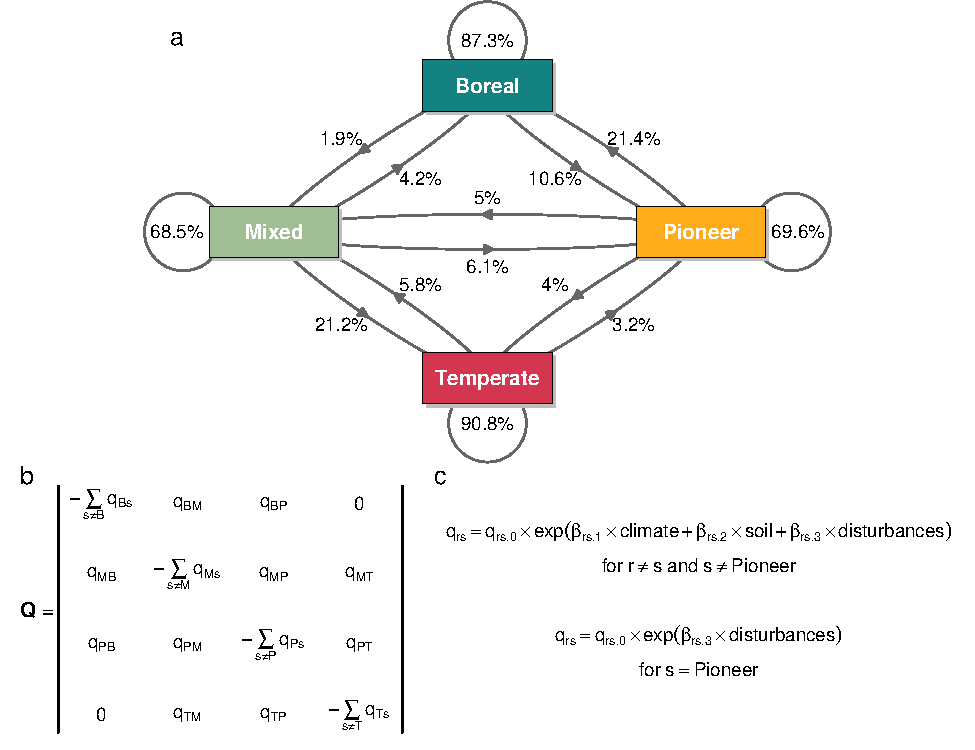
\includegraphics{res/fig2_trans_diagram.pdf}
\caption{Multi-state transition diagram (a), intensity matrix (b) and
equations of our full model (c). Directional arrows in (a) depict the
allowed transitions between states. The numbers represent the percentage
of observed transitions between states
(nb\textsubscript{rs}/nb\textsubscript{r.} x 100). Instantaneous
transition from Boreal to Temperate and vice versa are considered
impossible in the model (hence the absence of arrows in the diagram and
the zeros in the Q matrix), however rare transitions from Boreal to
Temperate and from Temperate to Boreal were observed in the data (less
than 0.2\%). All transitions from any states to Pioneer were modeled
only as dependent of disturbances.}
\end{figure}

\hypertarget{evaluation-of-candidate-models}{%
\subsubsection{Evaluation of candidate
models}\label{evaluation-of-candidate-models}}

We first evaluated the goodness-of-fit of each model containing
covariates (climate, soil, disturbances and full) against the baseline
model using likelihood ratio tests (Jackson, 2011), which test if the
addition of one or more new parameters significantly increases the
likelihood of the model. The statistical significance of individual
covariates in the presence of the other was determined by comparing the
full model with the correspondingly reduced model using likelihood ratio
tests.

\hypertarget{prediction-performance-of-candidate-models}{%
\subsubsection{Prediction performance of candidate
models}\label{prediction-performance-of-candidate-models}}

We fitted all models on the full data sets but also used
cross-validation to estimate the predictive performance on held-out
data. We used two statistics, the area under the receiver operating
characteristic (ROC) curve (AUC) and the logarithmic scoring rule (LS),
to assess the agreement between the observed state and the models'
predictions. The AUC is a popular performance metric for binary
classifiers that measures the probability of correct ranking of a random
positive-negative pair. The AUC ranges from 0 to 1, where a score of 1
indicates perfect discrimination, while a score of 0.5 is as good as
random. Hand \& Hill (2001) has extended the AUC method to multi-class
problems, here denoted mAUC. For any pair of states \(r\) and \(s\), we
can compute \(\hat{A}(r|s)\), the probability that a randomly drawn
member of state \(s\) has a lower estimated probability of belonging to
state \(r\) than a randomly drawn member of state \(r\). We can measure
the discrimination rate between all pairs of states by computing the
pairwise AUC:

\[\hat{A}(r,s) = [\hat{A}(r|s)+ \hat{A}(s|r)]/2\]

The mAUC can be obtained by averaging the pairwise AUC:

\[mAUC = \frac{2}{c(c-1)} \sum_{r<s} \hat{A}(r,s)\]

The LS was proposed by Good (1952) and is often used in weather
forecasts (Gneiting \& Raftery, 2007). While AUC is a function of
different classification thresholds, LS measures the degree to which
predicted probabilities are close to the observed outcomes. We computed
a global score for each model:

\[LS = \frac{1}{N} \sum_{i=1}^N -log(P(S_i = s_i))\]

where \(S_i\) is the random variable describing the state of the forest
in the \(i^{th}\) plot and \(s_i\) is the observed state. So, LS only
depends upon the predicted probability of the realized state and not on
the probabilities assigned to the other possible states. The score is
very sensitive to incorrect predictions: if a model predicted the
observed state with a probability of 100\%, the score for that plot is
0, while if a probability of zero was assigned to the observed state,
the score goes to infinity. Hence, this sensitivity allows to emphasize
the differences between model predictions and strongly penalize a model
that only gives high probabilities to self transitions.

To assess the quality of prediction for the four states individually, we
also computed LS for each state \(r\) where we summed the predicted
probability \(P(S_i = r)\) if the observed state is indeed \(r\) and
\(1 - P(S_i = r)\) otherwise.

We evaluated and compared the predictive performance of our five models
using the overall mAUC and the pairwise AUCs, as well as the overall LS
and the state-specific LS. These metrics were estimated using stratified
K-fold cross-validation {[}REF{]}. We first stratified the data set by
bioclimatic domain to ensure that each fold was representative of the
plot geographical distribution and randomly split the data set in k=10
folds. The cross-validation process was repeated k times, during which k
− 1 folds were used to train the models and the remaining fold was used
to validate the model predictions against the observed state
transitions. The cross-validated performance metrics were then averaged
for each model.

\hypertarget{effects-of-covariates-on-the-transition-dynamic}{%
\subsubsection{Effects of covariates on the transition
dynamic}\label{effects-of-covariates-on-the-transition-dynamic}}

Using the result from the best model, we compared the estimated hazard
ratios to investigate the influence of environmental covariates on
transition dynamic. We also computed the predicted 10-year transition
probabilities of forest plots under different disturbance scenarios,
while keeping all other covariates at their average found in the
ecotonal zone (i.e.~the balsam fir-yellow birch domain), to facilitate
visual interpretation of the impacts of disturbances on the matrix
structure.

To further understand how disturbances can modify the forest dynamic
under climate change, we characterized different properties of the
transition dynamic and compared them among levels and types of
disturbances along the latitudinal temperature gradient. An extensive
literature describes the multiple properties of discrete time Markov
transition matrix (Caswell, 2001; Hill et al., 2004) and these
properties can also be measured for continuous time Markov models. We
chose 4 informative and complementary properties that fully
characterized the dynamic of our modeled system: (1) the steady state
distribution, which corresponds to the long-term equilibrium state
distribution of the system; (2) the time of convergence to the steady
state; (3) the turnover time, which measures the speed of transient
successional changes; and (4) the entropy, which captures the
predictability of transitions.

First, we estimated the steady state distribution, \(\pi\). For a
regular Markov process, any initial state distribution \(s(0)\)
converges to the same equilibrium as \(t\) tends toward infinity:

\(\displaystyle \lim_{t \to \infty} s(0)P(t)=\pi\)

The vector of equilibrium \(\pi\) can be obtained by taking the left
eigenvector of \(Q\) with eigenvalue 0, normalized to sum to 1 or by
taking the dominant eigenvector of \(P\) with eigenvalue 1, normalized
to sum to 1 {[}REF{]}.

Then, the convergence rate to the equilibrium distribution can be
measured using the damping ratio (Hill et al., 2004):

\(\rho = \lambda_{P1} / \lambda_{P2}\) or
\(\rho = exp(\lambda_{Q1} - \lambda_{Q2})\),

where \(\lambda_{P1}\) and \(\lambda_{P2}\) are the largest and
second-largest eigenvalues of \(P\) (\(\lambda_{P1}\) = 1 for stochastic
\(P\)) and \(\lambda_{Q1}\) and \(\lambda_{Q2}\) are the largest and
second-largest eigenvalues of \(Q\) (\(\lambda_{Q1}\) = 0 for stochastic
\(Q\)). The half-life to equilibrium is given by:

\(t_{1/2} = log(2)/log(\rho)\)

We also measured the turnover time in each forest state, also called the
mean sojourn time in multi-state models, which corresponds to the time
spent in one state before transitioning to the next. The turnover time
can be estimated by \(Turnover_{r} =−1/q_{rr}\), where \(q_{rr}\) is the
r\^{}\{th\} entry on the diagonal of the estimated generator matrix. The
turnover of the whole system is given by the average of each state
turnover time over the steady state distribution:

\(Turnover = \displaystyle -\sum_r{\pi_r \times Turnover_{r}}\)

Finally, Hill et al. (2004) suggested using the entropy of a
discrete-time transition matrix as an index of the predictability of
successional changes. It measures how uncertain we are about the next
new state of a site knowing its current state. For a continuous-time
process, the entropy can be measured using the jump matrix (Spencer \&
Susko, 2005). The jump matrix contains the probabilities that the next
state after state \(r\) is state \(s\):

\(j_{rs} = −q_{rs}/q_{rr}\),

where \(qrs\) is the transition intensity from \(r\) to \(s\). The
entropy of state \(s\) is then:

\(H(j_{.s}) = \displaystyle -\sum_r{j_{rs} \times log(j_{rs})}\)

The normalized entropy of the whole system is the average of the
entropies over the steady state, divided by
\(H_{max} = log(n_{state} = 4)\):

\(\text{Entropy} = \displaystyle \frac{-\sum_r{\pi_r \times H(j_{.s})}}{H_{max}}\)

Values of entropy closer to zero indicated a more deterministic
transition dynamic and values closer to one indicated a more random
dynamic.

All analyses were performed using the R programming language version
3.5.1 (R Core Team, 2018). The list of R packages that have been used
throughout the analysis is provided in the Supporting Information (Table
S1). All the data used in the study, in addition to R scripts to
reproduce the analyses and the figures, will be made available online on
Github unpon manuscript acceptance.

\hypertarget{results}{%
\section{Results}\label{results}}

\emph{Note: standardize verb tense + add letters to panel figures}

\hypertarget{transition-dynamics}{%
\subsection{Transition dynamics}\label{transition-dynamics}}

In this study, there are a total of 38,091 surveys that were recorded
for the 10,388 forest plots. At the beginning of the surveys, there were
4567 forest plots assigned as Boreal, 1143 as Mixed, 2712 as Pioneer,
and 1966 as Temperate. At the end, there were 4795 Boreal plots, 1106
Mixed plots, 2176 Pioneer plots and 2311 Temperate plots (Fig. 2; Table
S2). A large fraction of Mixed forests transitioned to Temperate forests
(21.2\%) but few did the opposite (5.8\%). There were many transitions
between Boreal and Pioneer, but more Pioneer recovered to Boreal than
the reverse. Temperate and Boreal forests were generally more stable
(large fraction of forests did not transition) than Mixed and Pioneer
forests (Fig. 2).

\hypertarget{model-evaluation}{%
\subsection{Model evaluation}\label{model-evaluation}}

Overall, the full model including climate, soil and disturbance
variables had the best fit and predictive performance (Fig. 3; Table 2).
All variable subsets improved significantly the likelihood of the model
(all likelihood ratio tests were highly significant, p
\textless{}\textless{} 0.001; Table 2). Model evaluation using 10-fold
cross-validation revealed that including climate and disturbances
improved overall model predictive performance (mAUC and LS), while soil
variables had a negligible effect (Fig. 3). All models were good at
distinguishing Boreal from Temperate (high pairwise AUC). Soil variables
slightly help to predict Mixed and Temperate states. Including climate
variables help to distinguish Mixed from the other states, while
including disturbances help to distinguish Pioneer from the other
states, especially Boreal. Hereafter, all inferences about transition
probability parameters were derived from the full model.

\begin{figure}
\centering
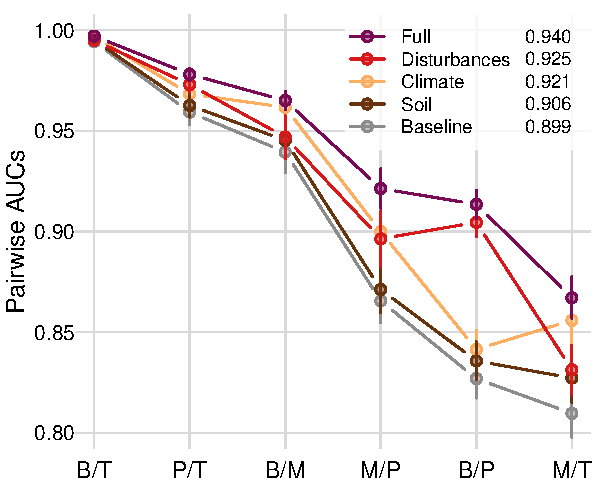
\includegraphics{res/fig3_cv_auc.pdf}
\caption{Mean pairwise AUC (areas under the receiver operating
characteristic curves) obtained through 10-fold cross-validation. Higher
values indicate a better capacity to discriminate between the four
forest states: (B)oreal, (M)ixed, (P)ioneer and (T)emperate. The overall
mAUC of each model is given next to the legend.}
\end{figure}

\textbf{AND/OR}

\begin{figure}
\centering
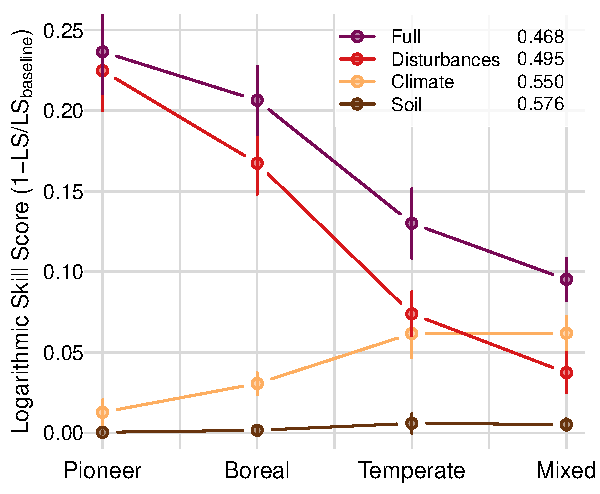
\includegraphics{res/fig3_cv_LSS.pdf}
\caption{Mean state-specific logarithmic skill score where each model
including covariates is compared to the baseline model. Values were
obtained through 10-fold cross-validation. Higher values indicate a
larger improvement (predicted probabilities are closer to the observed
outcomes) compared to the baseline model. The overall logarithmic score
of each model is given next to the legend.}
\end{figure}

\textbf{OR}

\begin{figure}
\centering
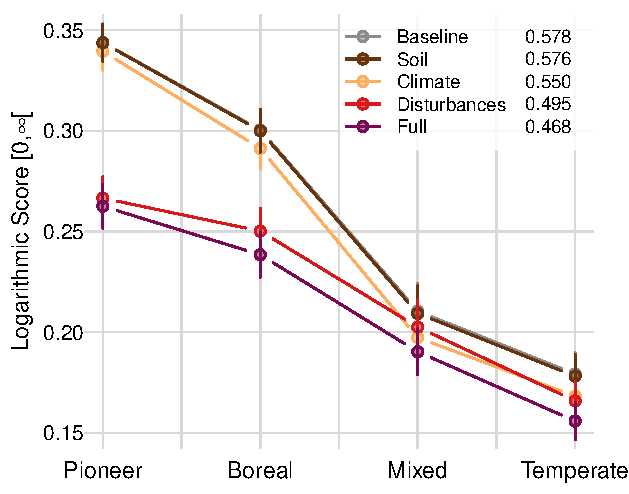
\includegraphics{res/fig3_cv_LS.pdf}
\caption{Mean state-specific logarithmic score obtained through 10-fold
cross-validation. Lower values indicate that the predicted probabilities
are closer to the observed outcomes. The overall logarithmic score of
each model is given next to the legend.}
\end{figure}

Table 2. Comparisons of the five candidate multi-state models. The
number of parameters used in each model corresponds to the number of
modeled transitions (10) \(\times\) the number of covariates. The
\(\Delta\)AIC is the difference between the Akaike information criterion
of each model (AIC\textsubscript{m}) and the minimum of AIC among all
the models (AIC\textsubscript{min}): \(\Delta\)AIC =
AIC\textsubscript{m} -- AIC\textsubscript{min}. Multi-class area under
the curve (mAUC) and logarithmic score were obtained through 10-fold
cross-validation. Higher mAUC and lower LS indicate better model
predictive performance. The best model is the one in bold with
\(\Delta\)AIC = 0.

\begin{longtable}[]{@{}llrrrrrr@{}}
\toprule
& Covariates & Nb of parameters & -2 Log-likelihood & \(\Delta\)AIC & LR
test & mAUC & LS\tabularnewline
\midrule
\endhead
Baseline & Intercept & 10 & 32032.3 & 6132.6 & \textless{} 0.001 & 0.899
& 0.578\tabularnewline
Climate & Temperature, CMI & 24 & 30438.7 & 4566.9 & \textless{} 0.001 &
0.921 & 0.550\tabularnewline
Soil & Drainage, pH & 24 & 31886.9 & 6015.2 & \textless{} 0.001 & 0.906
& 0.576\tabularnewline
Disturbances & Natural, Logging & 50 & 27341.3 & 1521.6 & \textless{}
0.001 & 0.925 & 0.495\tabularnewline
\textbf{Full} & \textbf{All} & \textbf{78} & \textbf{25763.7} &
\textbf{0.0} & \textless{} 0.001 & \textbf{0.940} &
\textbf{0.468}\tabularnewline
\bottomrule
\end{longtable}

\pagebreak

\hypertarget{effect-of-covariates-on-transition-intensity}{%
\subsection{Effect of covariates on transition
intensity}\label{effect-of-covariates-on-transition-intensity}}

The full multi-state model allows to reveal interesting relationships
between probabilities of forest state transition and environmental
covariates. All transitions to Pioneer were highly influenced by
disturbances (Fig. 4). As expected, major disturbances exert stronger
effects than moderate disturbances (for both natural and logging), but
logging had stronger effects for both levels of intensity. For example,
the risk of transition from Boreal to Pioneer has surged up to 165 times
higher for plots that suffered major logging (logging 2) compared to
that which were not disturbed (minor). Disturbances of all types and
intensities favored transitions from Mixed to Temperate forests. Major
disturbances increase the risk of transition from Mixed to Temperate by
ca. 5 times (Hazard Ratio (HR) = 4.51 and 5.32, for natural and logging,
respectively). Moderate disturbances (natural and logging) also favored
transitions from Boreal to Mixed (HR = 2.80 and 2.78, respectively),
while major disturbances had no significant effect.

Climate variables also had a significant influence on most transitions
(Fig. 4). Warmer summer temperature (higher sTP) and higher humidity
(higher CMI) favored the transitions from Boreal to Mixed as well as
from Pioneer to Mixed and Pioneer to Temperate. Interestingly, warmer
temperature did not significantly influence the risk of transition from
Mixed to Temperate and higher CMI had a negative effect.

Although less important (Fig. 3), soil variables also impacted state
transitions (Fig. 4). Holding the other covariates constant, poorer
drainage (more humid) decreased the instantaneous risk of transition
from Boreal to Mixed by 29\% and from Pioneer to Temperate by 17\%, but
increased the risk of transition from Temperate to Mixed by 32\% (HR =
0.71, 0.83 and 1.32, respectively). Higher pH (acidic soil) had a
considerable negative effect on the transitions from Temperate to Mixed
and a smaller one on transitions from Pioneer to Boreal (HR = 0.80 and
0.93, respectively). These changes in risk ratio associated to soil
variables appear almost irrelevant compare to the effect of
disturbances, but a slight increase in drainage can dampen the positive
effect of disturbances. For instance, under moderate natural
disturbances, the estimated risk of transition from Boreal to Mixed is
2.12 (1.04-4.33) at moderate drainage but decreases to 1.50 (0.71-3.20)
when increasing drainage by 1 point.

\begin{figure}
\centering
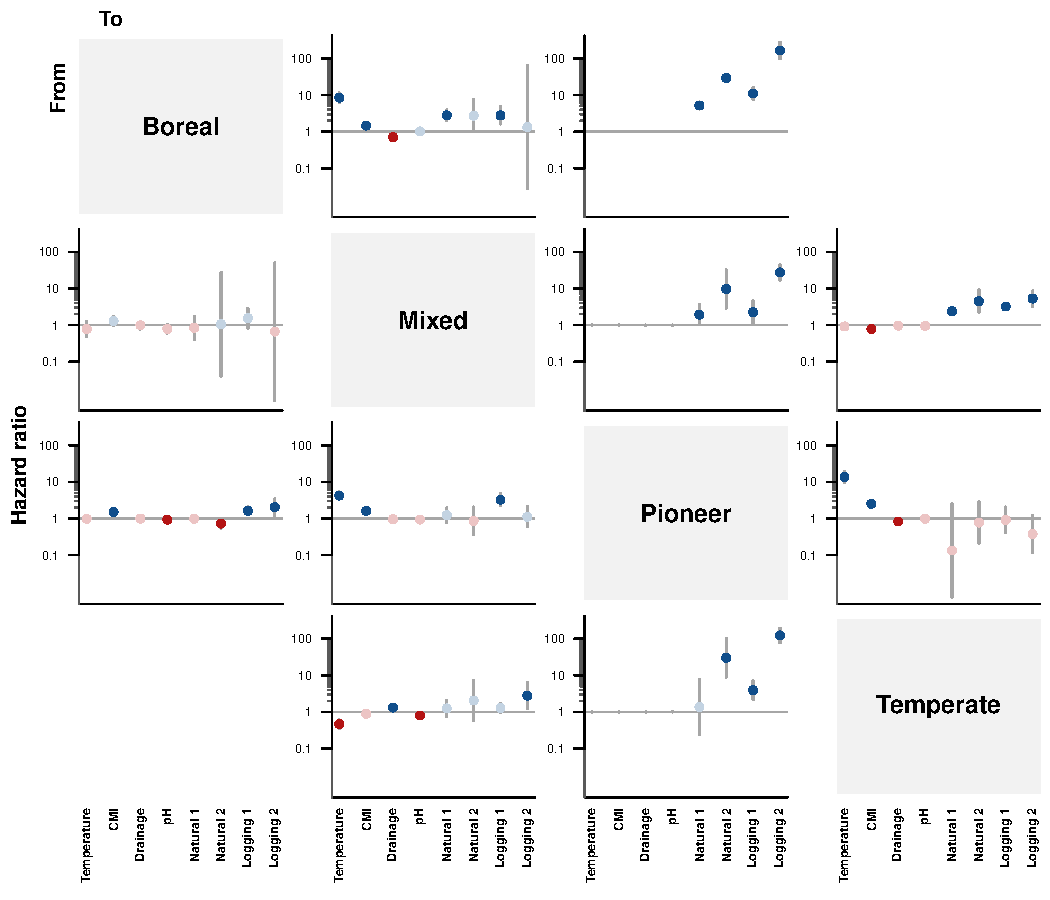
\includegraphics{res/fig4_HR.pdf}
\caption{Hazard ratios (HR) and 95\% confidence intervals as estimated
from the best multi-state transition model. The y-axis is in log scale.
The HR of predictors are interpretable as multiplicative effects on the
hazard, where values above 1 (in blue) indicate that the predictor is
associated with a greater risk of state transition, while values below 1
(in red) indicate a lower risk of transition. Predictors different from
1 are colored in dark blue or red. Numbers following disturbance
predictors indicate their levels of intensity: 1 = moderate and 2 =
major.}
\end{figure}

\pagebreak

Disturbances completely altered the structure of the 10-year transition
probability matrix (Fig. 5). The largest values across most matrices
were generally associated with self transitions (matrix diagonal),
meaning that the vast majority of forest plots (characterized by the
average environmental conditions of ecotone) remain in the same state
after 10 years. For undisturbed forest plots (minor), the self
transitions are very strong but transitions from Pioneer to Boreal, from
Mixed to Temperate, and from Temperate to Mixed were not trivial. At
moderate disturbances, probabilities of self transitions decrease, while
transitions from Boreal to Pioneer, from Mixed to Temperate increase the
most. Transitions from Mixed and Temperate to Pioneer do not increase
much at moderate disturbances, likely because such disturbances were
less frequent and less severe than in Boreal forests. The difference
between natural disturbances and logging emerges only at major
disturbances. For both types of major disturbances, the probabilities in
the third column, transitions to Pioneer, showed a great increase
compare to moderate disturbances, but these values exploded in severely
logged transition matrix, exceeding self transitions. Interestingly, the
estimated probability of Mixed to Temperate remain quite high at major
disturbances.

\begin{figure}
\centering
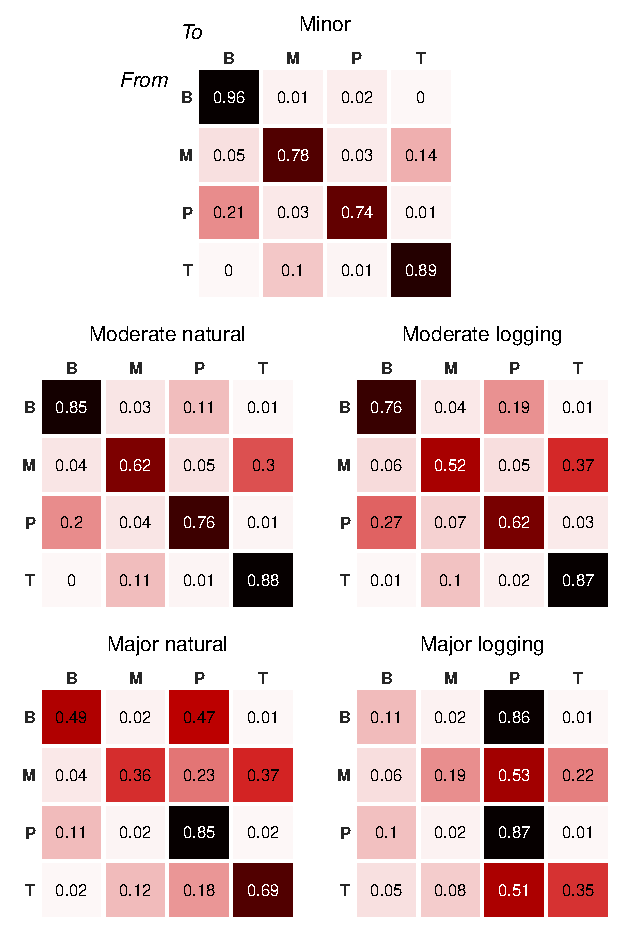
\includegraphics{res/fig5_pmatrix.pdf}
\caption{Predicted change in 10-year transition probabilities for
different disturbance types and levels. All other covariates are fixed
at the average conditions found in the ecotone, i.e.~the balsam
fir-yellow birch domain. Letters correspond to the four forest states:
(B)oreal, (M)ixed, (P)ioneer and (T)emperate. Numbers are the modeled
transition probabilities from rows to columns and darker color
highlights stronger transitions.}
\end{figure}

\pagebreak

\hypertarget{effect-of-disturbances-on-long-term-equilibrium}{%
\subsection{Effect of disturbances on long term
equilibrium}\label{effect-of-disturbances-on-long-term-equilibrium}}

The steady state forest dominance changes as expected along the
temperature gradient (Fig. 6); the Boreal state dominates at low
temperature (high latitude) and Temperate and Mixed states dominate at
high temperature (low latitude), with a transition boundary located at a
growing season temperature of about 12.75°C, which falls in the ecotonal
balsam fir-yellow birch domain. When moderate disturbances were
included, the steady state proportion of Temperate and Mixed forests
increases and the Boreal-Temperate boundary occurred at lower
temperatures, hence further north in the balsam fir-white birch domain
(Fig. 6). Moderate natural disturbances and logging had a similar
positive effect on the proportion of Temperate and Mixed. For example,
at 12.58°C, northern end of balsam fir-yellow birch domain, the steady
state proportion of Temperate and Mixed almost doubles with moderate
disturbances (minor: 36\%; moderate natural: 58\%; moderate logging:
60\%). However, because there was a larger reduction in the proportion
of Boreal to the benefit of Pioneer, the displacement of the boundary
was slightly larger for logging than natural disturbances (displaced at
12.05°C for logging and at 12.18°C for natural disturbances; Fig. 6).
Finally, for major disturbances, the proportion of Boreal forests at
steady state collapsed while that of Temperate and Mixed forests also
decreased to a lesser extent. The landscape is now dominated by Pioneer
forests. The boundary modestly moved north with major natural
disturbances (12.60°C), while it retreated to the south with major
logging (13.05°C). Simulating change in frequency of disturbances
(instead of all or nothing scenarios) shows that the Boreal-Temperate
boundary slowly moved north with increasing moderate disturbance
frequency (natural or logging), but it stagnates with increasing
frequency of major natural disturbances and recedes south with
increasing frequency of major logging (Fig. S3).

\begin{figure}
\centering
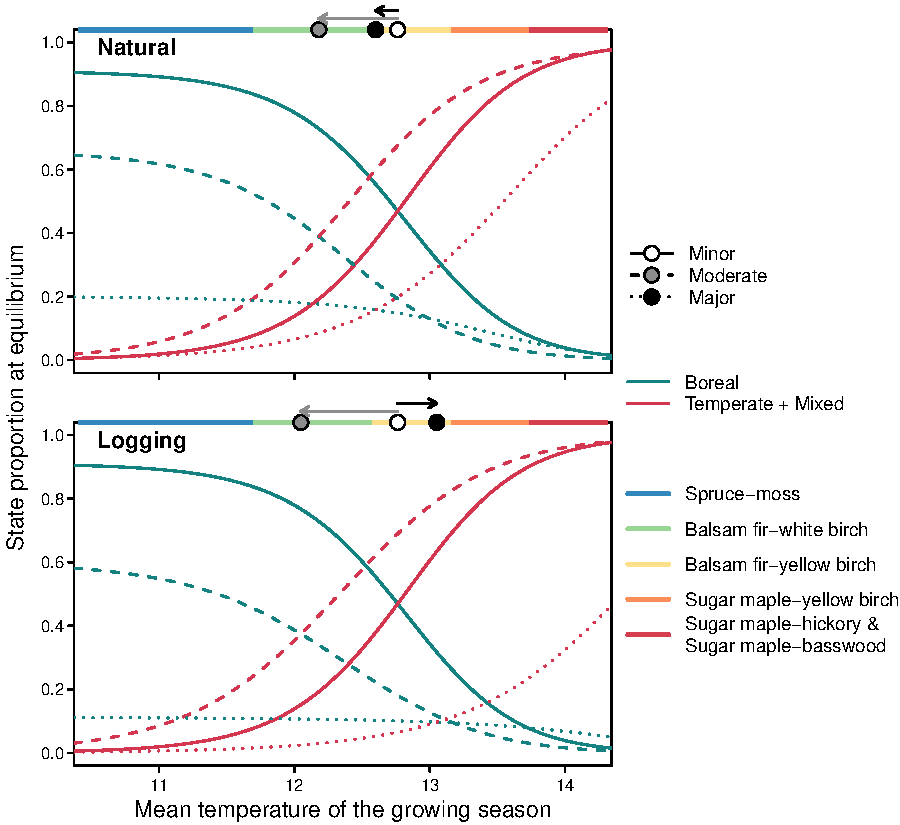
\includegraphics{res/fig6_SS_gradient.pdf}
\caption{Changes in forest state proportion at equilibrium along the
temperature (latitudinal) gradient for different disturbance scenarios.
Proportion of Boreal (blue) and Temperate + Mixed forests (red) for
minor (solid), moderate (dashed) and major (dotted) disturbances. All
other covariates are fixed at the average conditions found in the
ecotone, i.e.~the balsam fir-yellow birch domain, to focus solely on the
effect of disturbances along the temperature gradient. The white
(minor), grey (moderate) and black (major) circles indicate the position
of the boundary between dominance of Boreal forests and dominance of
Temperate and Mixed forests (i.e.~the advancing front). The colors at
the top of the plots approximate the position of the bioclimatic domains
along the temperature gradient.}
\end{figure}

\hypertarget{effect-of-disturbances-on-transient-dynamics}{%
\subsection{Effect of disturbances on transient
dynamics}\label{effect-of-disturbances-on-transient-dynamics}}

Natural disturbances and logging affected forest transient dynamics,
with greater impacts for higher disturbance intensity (Fig. 7). In the
minor disturbance scenario, turnover time was generally longer at low
temperature, indicating a slow transition dynamic in forests of northern
latitudes (Fig. 7a,b). The turnover time then rapidly declines to reach
a minimum at 13.20°C, between the sugar maple-yellow birch and the
balsam fir-yellow birch domains, and goes back up after this point. This
trough, where transition dynamics are the fastest, is located just a
little south of the point of transition between Boreal and Temperate
dominance found in Figure 6. Major disturbances accelerate transition
dynamics all along the temperature gradient, while moderate disturbances
also decrease turnover time but more strongly in the boreal domains
(balsam fir-white birch and spruce-moss domains; Fig. 7a,b). These
spatial patterns reflect the turnover time of the dominant state at each
point along the temperature gradient (Fig. S4).

At minor disturbances, the entropy of the system generally increases
from north to south and peaked at 12.56°C, at the southern end of the
balsam white-birch domain (Fig. 7c,d). This peak illustrates where the
transition dynamic is most uncertain (transition to all states are
possible at this point), while it is very predictable in northern boreal
forests (Boreal stays Boreal until it transitions to Pioneer later on).
The peak can be mainly attributed to the entropy of the Boreal state and
the generally high values at high temperature can be principally
attributed to the Temperate state (Fig. S5). This latitudinal pattern of
entropy is modified by disturbances. Moderate natural disturbances
decrease the entropy throughout the gradient, but especially where was
the peak (Fig. 7c). With moderate logging, the peak disappears and
entropy increases monotonically from north to south (Fig. 7d). When
major disturbances are included, wether natural or logging, the peak of
entropy is displaced to the south (Fig. 7c,d) where it is dominated by
the entropy of the Pioneer state (Fig. S5).

The half-life to equilibrium is the longest at 12.24°C, in the balsam
fir-white birch domain, while it is the fastest in the southernmost
latitudes (Fig. 7e,f). Interestingly, the peak for half-life closely
matches the peak for entropy, but matches no feature of the turnover
time curve. Moderate disturbances flatten and shift this peak to the
north and the effect of moderate logging (Fig. 7f) is stronger than
natural disturbances (Fig. 7e). Hence, in the balsam fir-white birch,
the half-life to reach equilibrium distribution is reduced almost by
half by moderate logging. With major disturbances, forests all along the
temperature gradient can reach very quickly their steady state
distribution (maximum of about 8 years for major logging and 25 years
for major natural disturbances).

\begin{figure}
\centering
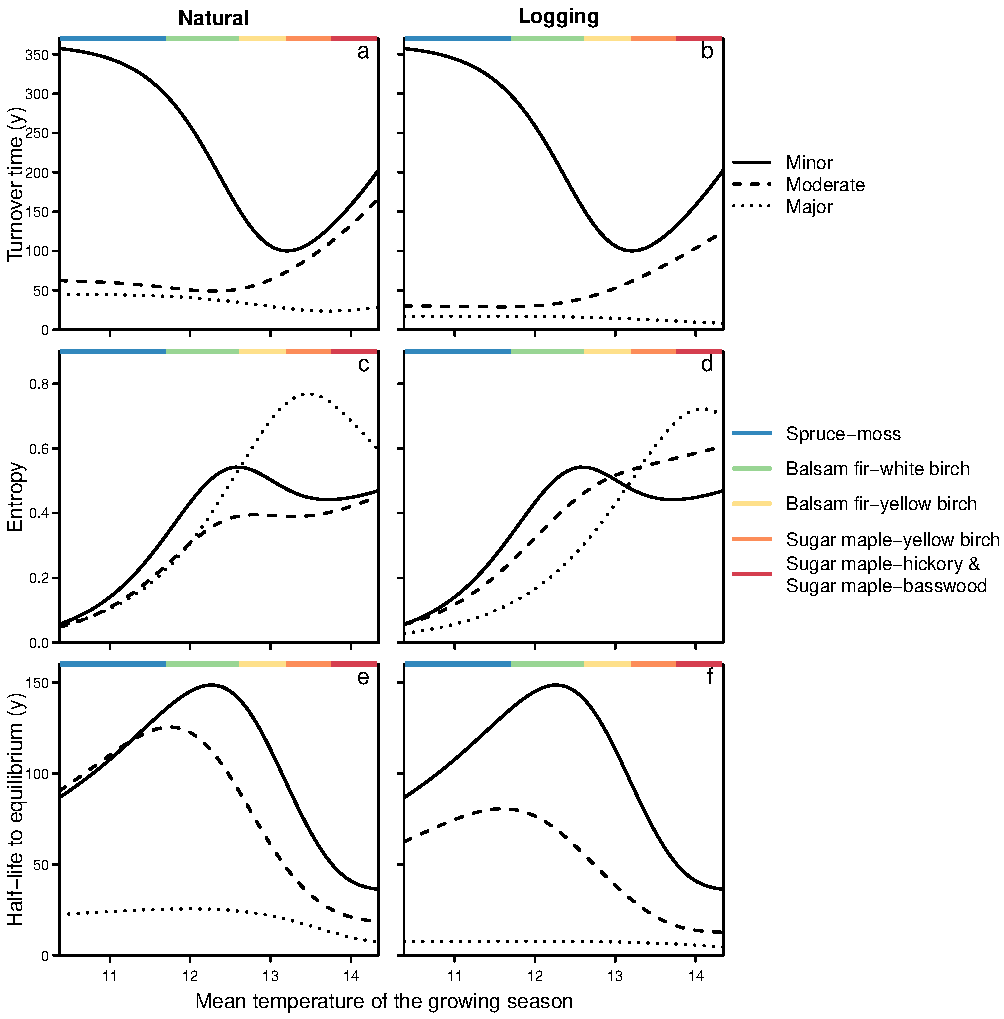
\includegraphics{res/fig7_index_gradient.pdf}
\caption{Changes in the characteristics of the forest transient dynamics
along the temperature (latitudinal) gradient for different disturbance
scenarios: minor (solid), moderate (dashed) and major (dotted)
disturbances for both natural (a,c,e) and logging (b,d,f). All other
covariates are fixed at the average conditions found in the ecotone,
i.e.~the balsam fir-yellow birch domain, to focus solely on the effect
of disturbances along the temperature gradient. The turnover of the
whole system (i.e.~whole transition matrix) (a,b) corresponds the time
spent in a state before transitioning to the next and is given by the
average of each state turnover time over the steady state distribution.
The entropy of the whole system (c,d) corresponds to the incertitude of
the next transition and is given by the average of each state entropy
over the steady state distribution. The half-life to equilibrium (e,f)
is the time taken to reach 50\% of the steady state distribution,
i.e.~when the first eigenvalue to become twice as great as the
contribution of the second eigenvalue. The colors at the top of the
plots approximate the position of the bioclimatic domains.}
\end{figure}

\hypertarget{discussion}{%
\section{Discussion}\label{discussion}}

\hypertarget{p1.-main-results}{%
\subsection{P1. Main results}\label{p1.-main-results}}

Our study reveals that disturbances are likely to accelerate forest
response to climate change by promoting transitions from boreal to mixed
forests and, particularly, from mixed to temperate forests. Our analysis
of the equilibrium further highlights that the long term forest dynamics
under moderate disturbances favors an increase proportion of temperate
forests and a northward shift of the boreal-temperate ecotone.
Disturbances also modified the forest transient dynamics, accelerating
both the turnover and convergence time and making the dynamics more
predictable. In accordance with the hypothesis formulated by previous
studies (Brice et al., 2019; Johnstone et al., 2016, 2010; Vissault,
2016), our findings demonstrate that moderate disturbances catalyze
transition to alternate, temperate-dominated forest state and, as a
result, promote regime shifts.

\hypertarget{p2.-is-forest-transition-dynamic-affected-by-recent-climate-change}{%
\subsection{P2. Is forest transition dynamic affected by recent climate
change?}\label{p2.-is-forest-transition-dynamic-affected-by-recent-climate-change}}

Our results seem to support the hypothesis that recent climate warming
influences transition dynamics among forest states at the
boreal-temperate ecotone. The higher number of transitions from mixed to
temperate is consistent with the expectation of a northward shift in
range of temperate trees species into the mixed and boreal forests.
Indeed, the warming trends of the last decades (fig supp?) have been
shown to improve growth and reproductive rates of temperate species, but
to reduce growth of boreal species (Boisvert‐Marsh, Périé, \& Blois,
2019; Fisichelli et al., 2014; Goldblum \& Rigg, 2005; Reich et al.,
2015), thus providing a competitive advantage of temperate over boreal
species.

Alternatively, the increased transition to temperate species may be a
response to other pressures. Comparisons of pre-settlement and
present-day forested landscape of North America have demonstrated an
important deciduous encroachment in response to historical human
activities (Boucher, Arseneault, \& Sirois, 2006; Danneyrolles et al.,
2019; Terrail et al., 2019). Similarly, Johnstone \& Chapin (2003)
suggests that the northern range expansion of lodgepole pine following
fire is not related to current climate change, but was rather a
continued migration initiated in the early Holocene. However, historical
legacies and climate change are likely mutually non-exclusive
explanations. Simulations by Boulanger et al. (2019) showed that the
future climate-induced expansion in temperate species to the detriment
of boreal species would amplify the already ongoing trend since
preindustrial times.

\hypertarget{p3.-environmental-catalysts-and-inhibitors-of-forest-state-transition}{%
\subsection{P3. Environmental catalysts and inhibitors of forest state
transition}\label{p3.-environmental-catalysts-and-inhibitors-of-forest-state-transition}}

Our study demonstrated that moderate disturbances favor climate-related
transitions, while major disturbances merely promote pioneer states.
Disturbances directly remove trees which lead to immediate and
substantial changes in forest composition and successional trajectories.
Without climate change, forests are expected to be resilient to normally
experienced disturbances and should thus return to their previous
states. However, climate change alters the conditions that initially
supported the persistence of a forest state, making them more vulnerable
to disturbances (Johnstone et al., 2016). Hence, moderate disturbances
remove resident species and reduce competition for light and nutrient,
which likely facilitate colonization and establishment by opportunistic
temperate species under warmer conditions (Brice et al., 2019;
Landhäusser et al., 2010; Leithead et al., 2010). In contrast, severe
disturbances in the study area, primarily clearcutting but also large
fires, create openings of very large extent which likely favor
early-successional species that can disperse seed over long distances,
such as \emph{Populus sp} and \emph{Betula sp} (Landhäusser et al.,
2010).

Compared to the catalyzing effect of disturbances, soil characteristics
do not appear as a large impediment to state transition but have the
potential to slow down transitions. Poor drainage constrained
climate-related transitions, from Boreal to Mixed states, but not from
Mixed to Temperate. This indicates that temperate species can readily
colonize soils found in mixedwoods, but may have more difficulty to
colonize hydric boreal soils. Very poor drainage, often associated with
peatland and thick organic layer, is indeed considered as one of the
only major edaphic limit for the regeneration of temperate species
(Lafleur et al., 2010). Numerous studies found that \emph{Acer
saccharum} regenerate well across the ecotone because of its large
tolerance to various soil conditions (Barras \& Kellman, 1998; Collin,
Messier, Kembel, \& Bélanger, 2018; Fisichelli et al., 2014; Goldblum \&
Rigg, 2002; Kellman, 2004). At their northern range limit, \emph{A.
saccharum} and \emph{A. rubrum}, the species contributing most to
compositional changes (Brice et al., 2019), are hypothesized to be
mostly limited by soil temperature (Barras \& Kellman, 1998; Goldblum \&
Rigg, 2002).

Moreover, disturbances may counteract any effect of soil properties.
Indeed, disturbances, such as logging and fire, often remove the surface
organic layers and expose mineral soil and can, consequently, provide an
appropriate seedbed for temperate species recruitment (Archambault,
Delisle, Larocque, Sirois, \& Belleau, 2006; Landhäusser et al., 2010).
In combination with climate warming, disturbances may also facilitate
temperate migration by increasing understory air and soil temperatures
(De Frenne et al., 2013; Stevens, Safford, Harrison, \& Latimer, 2015).

\hypertarget{p4.-equilibrium-and-potential-range-limits}{%
\subsection{P4. Equilibrium and potential range
limits}\label{p4.-equilibrium-and-potential-range-limits}}

Our model highlights the potential role of disturbances in controlling
the position of the boreal-temperate boundary as well as the proportion
of temperate and boreal biomes at equilibrium. As a result of the
increased replacement of Mixed by Temperate states and a decline of
Boreal to Pioneer states, the equilibrium boreal-temperate boundary
shifts northward with moderate disturbances. While our results should
not be interpreted as predictions of the future, they are useful to
highlight the direction of the forest dynamic. Our results support the
simulations of Boulanger et al. (2019) where harvesting under future
climate warming was projected to promote further invasions of pioneer
species, such as \emph{Populus}, and temperate species, such as
\emph{Acer} and \emph{Fagus}, in mixedwoods of Québec. In contrast,
based on their simulations, Liang et al. (2018) and Vanderwel \& Purves
(2014) concluded that logging would accelerate the expansion of pioneer
forests, but have little or no effect on extensive biome shifts over the
next century in eastern United States. These apparently conflicting
results could be due to the contrasting tree species responses to
disturbance. Disturbances may facilitate the range expansion of some
species but hinder that of others depending on their functional traits
(Aubin et al., 2016; Matthews, Marsh-Matthews, Cashner, \& Gelwick,
2013). For instance, because of its positive response to past
(Danneyrolles et al., 2019), recent (Brice et al., 2019) and future
(Boulanger et al., 2019) disturbances in Québec, \emph{Acer rubrum} is
likely to play a disproportional role in the temperate biome shift.

\begin{itemize}
\item
  *Can we really compare?
\item
  in all disturbance scenarios, boreal forests are losing ground
  primarily to pioneer forests
\item
  Similar to Liang et al. (2018) and Vanderwel \& Purves (2014) We also
  predict that major disturbances will only promote pioneer states to
  the detriment of boreal states\ldots{}
\end{itemize}

Other results: Simulations by Vieira showed that plantation and
enrichment planting shifted northward the boreal-temperate range limits,
but not harvesting. Thinning increased the transition from mixed to
temperate stands, but did not have any effect on range limits shift.

Boulangeat et al. (2018) even predicted a southern shift of the
boreal-temperate boundary when including the effects of herbivores.*

\hypertarget{p5.-transient-dynamics}{%
\subsection{P5. Transient dynamics}\label{p5.-transient-dynamics}}

\emph{Help! Not sure how to interpret these results!}

Beyond their impacts on steady state distribution, our results suggest
that disturbances may have a substantial influence on forest transient
dynamics. In the continuous boreal zone (spruce-moss domain), forests
dominated by \emph{Picea mariana} are usually characterized by a dynamic
of stand self replacement with minimal compositional changes across
disturbance cycles (Goldblum \& Rigg, 2010). Consistent with this
dynamic, the turnover time of undisturbed northern boreal forests is
very long and the entropy very low. The turnover becomes very rapid with
disturbances, but the entropy remains low indicating that the dynamic is
still as predictable (back and forth transitions between boreal and
pioneer states) and that there is no shift dynamic associated with
disturbances. Hence, while resistant at low disturbances, boreal forests
loose their resistance when moderately disturbed but remain resilient as
they return to their previous boreal state. Under major disturbances,
boreal forests collapse to pioneer state and reach this new equilibrium
swiftly (short half-life). This interpretation agrees with previous
studies suggesting that boreal forests can easily shift into an
alternative treeless state in response to severe or repeated
disturbances (Payette \& Delwaide, 2003; Sánchez-Pinillos et al., 2019).

In contrast, the ecotone is characterized by a rapid turnover and a high
entropy indicating abrupt compositional shift which can go in all
directions, hence this zone is neither resistant nor resilient. Compared
to northern boreal forests, the short turnover time implies a low
persistence, hence a low resistance, of the forest states in this region
even under minor disturbances. This result corroborate the predictions
made by Vissault (2016), where mixed forests undergo a swift conversion
to temperate forests in the next decades whereas boreal forests present
a large amount of inertia. The dynamic of the ecotone appear unstable
because it is caught between the two stable states, i.e. boreal to the
north and temperate to the south. Under moderate disturbances, the
probability of transitioning to Temperate increases to the detriment of
the other possible states (Fig. 6), hence the entropy is decreased and
the dynamic becomes more predictable. Such a clear directional shift
strongly indicates a non‐equilibrium dynamic in this region. Although
turnover is fast, half-life to equilibrium is long because a forest may
not move in the right direction and may undergo multiple transitions.

\begin{itemize}
\item
  *implication for resilience and resistance

  \begin{itemize}
  \tightlist
  \item
    long turnover = high persistence = high resistance?
  \item
    high entropy = low stability/resilience?
  \end{itemize}
\item
  Compare to Boulangeat et al. (2018) + Vieira -In contrast to our
  results, Boulangeat et al. (2018) showed that disturbances by browsers
  ``reduced the asymptotic resilience of the system, decreasing the rate
  at which the new equilibrium was approached.'' Effect of browsers are
  likely less dramatic than tree logging (here moderate disturbances
  remove at least 25\% of the basal area).
\item
  active migration zone more sensitive
\item
  at this scale there appear to be no difference between natural and
  anthropogenic disturbances.*
\end{itemize}

\hypertarget{p6.-limitations-of-the-study}{%
\subsection{P6. Limitations of the
study}\label{p6.-limitations-of-the-study}}

Our goal was not to make predictions about the future state of Québec
forests, but rather to explore how disturbances and soils may interact
with recent climate change and modify transition dynamics. For this
reason, it is inappropriate to regard the state distribution at
equilibrium or the half-life to convergence as specific predictions
about the extent and timing of biome shifts. Indeed, we did not simulate
future climate change, we have only considered recent climate change
that was observed during the surveyed period. Moreover, we did not
include any dispersal limitations, although it is known to affect tree
migration (Pearson, 2006). Because detailed temporal data on tree
composition around each plot is not available, neighborhood composition
should have been approximated using climate data, but we considered that
it was redundant as they are already used in our multi-state model.
Dispersal limitations could potentially reduce the effect of
disturbances on long term forest distribution, but should not influence
our empirically derived results.

Finally, the definition of states can affect to some extent the results.
A higher threshold to define the boreal and temperate states (e.g.,
\textgreater{}90\% instead of \textgreater{}75\% of dominance of boreal
and temperate, respectively) would change the transition probability but
the direction of the dynamic would remain the same.

\hypertarget{p7.-ecological-and-management-implications}{%
\subsection{P7. Ecological and management
implications}\label{p7.-ecological-and-management-implications}}

The relationships that we demonstrate between forest state transitions
and disturbances provide a strong empirical basis for predicting the
types of changes in forest dynamics that are likely to unfold in the
coming century. A shift in dominant forest cover from conifer to
deciduous broadleaf species not only entail changes in tree species
diversity and composition, but a complete transformation of forest
dynamics and functions. In the long term, this regime shift could
locally increase tree diversity and productivity {[}REF{]}, increase
carbon sequestration (Thurner et al., 2014; as long as mortality is
limited NRDC, 2018), modify disturbance regime (reduced flammability of
broadleaf species, Terrier, Girardin, Rie, Legendre, \& Bergeron, 2013
and reduced sensitivity to current outbreak-prone pest,
@mffp\_insectes\_2018), alter soil microbial activities (e.g. Laganière,
Paré, \& Bradley, 2010) and affect wildlife distribution (e.g. Mizel,
Schmidt, Mcintyre, \& Roland, 2016). However, such regime shift also
have large repercussions on forest management strategies in area where
silvicultural practices are tailored to regional disturbance regimes and
rely on natural regeneration.

Our study reveals the potential of moderate disturbances to facilitate
climate-related transitions and thus suggests that alternative
silvicultural practices could be used to reduced tree migration lags.
But even well planned logging may not benefit all species equally (Brice
et al., 2019) and may interact will other natural disturbances to
exacerbate tree mortality and compromise forest resilience in the long
run (Buma \& Wessman, 2011). In addition to alternative silvicultural
strategies, some studies suggest that temperate species could be planted
farther north to speed up succession {[}Iverson \& McKenzie (2013);
Duveneck \& Scheller (2016); Vieira et al.{]}. However, whether
promoting temperate tree migration is ``desirable'' or not depends on
the decisions we make regarding forest management. Do we try to maintain
historical conditions, let nature takes its course, or actively move
species to climatically suitable locations outside their current ranges
(Frelich \& Reich, 2010)? In Québec, ecosystem-based forest management
seek to maintain the composition and structure of a reference state,
define by the preindustrial forest conditions (Pinna, Québec (Province),
Ministère des ressources naturelles et de la faune, \& Consortium en
foresterie Gaspésie-Les-Îles, 2009). Yet, Boulanger et al. (2019) showed
that such management would fail to restore or approach historical forest
conditions under future climate change. In the context of ongoing
climate change, our study reinforces that forest management have to
consider the present system state in relationship to its transient
dynamic as well as its likely trajectory. But even then, simulations by
Duveneck \& Scheller (2016) suggest that alternative management
strategies, including modified silviculture and climate suitable
planting, will have limited ability to increase resilience and
resistance of forest under climate change. Therefore, in order to insure
long term forest resilience at the boreal-temperate ecotone, adaptative
management does not appear sufficient and drastic reduction of
greenhouse gas emission is necessary to limit global warming (IPCC,
2014).

\hypertarget{references}{%
\subsection*{References}\label{references}}
\addcontentsline{toc}{subsection}{References}

\hypertarget{refs}{}
\leavevmode\hypertarget{ref-archambault_fifty_2006}{}%
Archambault, L., Delisle, C., Larocque, G. R., Sirois, L., \& Belleau,
P. (2006). Fifty years of forest dynamics following diameter-limit
cuttings in balsam fir -- yellow birch stands of the Lower St. Lawrence
region, Quebec. \emph{Canadian Journal of Forest Research},
\emph{36}(11), 2745--2755. \url{https://doi.org/10.1139/x06-179}

\leavevmode\hypertarget{ref-aubin_traits_2016}{}%
Aubin, I., Munson, A., Cardou, F., Burton, P., Isabel, N., Pedlar, J.,
\ldots{} McKenney, D. (2016). Traits to stay, traits to move: A review
of functional traits to assess sensitivity and adaptive capacity of
temperate and boreal trees to climate change. \emph{Environmental
Reviews}, \emph{24}(2), 164--186.
\url{https://doi.org/10.1139/er-2015-0072}

\leavevmode\hypertarget{ref-barras_supply_1998}{}%
Barras, N., \& Kellman, M. (1998). The supply of regeneration
micro-sites and segregation of tree species in a hardwood/boreal forest
transition zone. \emph{Journal of Biogeography}, \emph{25}(5), 871--881.
\url{https://doi.org/10.1046/j.1365-2699.1998.00232.x}

\leavevmode\hypertarget{ref-bennett_plant-soil_2017}{}%
Bennett, J. A., Maherali, H., Reinhart, K. O., Lekberg, Y., Hart, M. M.,
\& Klironomos, J. (2017). Plant-soil feedbacks and mycorrhizal type
influence temperate forest population dynamics. \emph{Science},
\emph{355}(6321), 181--184.
\url{https://doi.org/10.1126/science.aai8212}

\leavevmode\hypertarget{ref-boisvertmarsh_divergent_2019}{}%
Boisvert‐Marsh, L., Périé, C., \& Blois, S. de. (2019). Divergent
responses to climate change and disturbance drive recruitment patterns
underlying latitudinal shifts of tree species. \emph{Journal of
Ecology}, \emph{0}(0). \url{https://doi.org/10.1111/1365-2745.13149}

\leavevmode\hypertarget{ref-boisvert-marsh_shifting_2014}{}%
Boisvert-Marsh, L., Périé, C., \& de Blois, S. (2014). Shifting with
climate? Evidence for recent changes in tree species distribution at
high latitudes. \emph{Ecosphere}, \emph{5}(7), art83.
\url{https://doi.org/10.1890/ES14-00111.1}

\leavevmode\hypertarget{ref-boucher_logging-induced_2006}{}%
Boucher, Y., Arseneault, D., \& Sirois, L. (2006). Logging-induced
change (1930-2002) of a preindustrial landscape at the northern range
limit of northern hardwoods, eastern Canada. \emph{Canadian Journal of
Forest Research}, \emph{36}(2), 505--517.
\url{https://doi.org/10.1139/x05-252}

\leavevmode\hypertarget{ref-boulangeat_transient_2018}{}%
Boulangeat, I., Svenning, J.-C., Daufresne, T., Leblond, M., \& Gravel,
D. (2018). The transient response of ecosystems to climate change is
amplified by trophic interactions. \emph{Oikos}, \emph{127}(12),
1822--1833. \url{https://doi.org/10.1111/oik.05052}

\leavevmode\hypertarget{ref-boulanger_climate_2019}{}%
Boulanger, Y., Arseneault, D., Boucher, Y., Gauthier, S., Cyr, D.,
Taylor, A. R., \ldots{} Dupuis, S. (2019). Climate change will affect
the ability of forest management to reduce gaps between current and
presettlement forest composition in southeastern Canada. \emph{Landscape
Ecology}, \emph{34}(1), 159--174.
\url{https://doi.org/10.1007/s10980-018-0761-6}

\leavevmode\hypertarget{ref-brice_disturbances_2019}{}%
Brice, H., Cazelles, K., Legendre, P., \& Fortin, J. (2019).
Disturbances amplify tree community responses to climate change in the
temperate--boreal ecotone. \emph{Global Ecology and Biogeography}, 14.

\leavevmode\hypertarget{ref-brown_non-climatic_2014}{}%
Brown, C. D., \& Vellend, M. (2014). Non-climatic constraints on upper
elevational plant range expansion under climate change.
\emph{Proceedings of the Royal Society B: Biological Sciences},
\emph{281}(1794), 20141779--20141779.
\url{https://doi.org/10.1098/rspb.2014.1779}

\leavevmode\hypertarget{ref-buma_disturbance_2011}{}%
Buma, B., \& Wessman, C. A. (2011). Disturbance interactions can impact
resilience mechanisms of forests. \emph{Ecosphere}, \emph{2}(5), art64.
\url{https://doi.org/10.1890/ES11-00038.1}

\leavevmode\hypertarget{ref-caswell_matrix_2001}{}%
Caswell, H. (2001). \emph{Matrix population models: Construction,
analysis, and interpretation} (2nd ed). Sunderland, Mass: Sinauer
Associates.

\leavevmode\hypertarget{ref-caswell_matrix_2008}{}%
Caswell, H. (2008). \emph{Matrix population models: Construction,
analysis, and interpretation} (2. ed., {[}Nachdr.{]}). Sunderland, Mass:
Sinauer Associates.

\leavevmode\hypertarget{ref-collin_conifer_2017}{}%
Collin, A., Messier, C., \& Bélanger, N. (2017). Conifer Presence May
Negatively Affect Sugar Maple's Ability to Migrate into the Boreal
Forest Through Reduced Foliar Nutritional Status. \emph{Ecosystems},
\emph{20}(4), 701--716. \url{https://doi.org/10.1007/s10021-016-0045-4}

\leavevmode\hypertarget{ref-collin_can_2018}{}%
Collin, A., Messier, C., Kembel, S. W., \& Bélanger, N. (2018). Can
sugar maple establish into the boreal forest? Insights from seedlings
under various canopies in southern Quebec. \emph{Ecosphere},
\emph{9}(1), e02022. \url{https://doi.org/10.1002/ecs2.2022}

\leavevmode\hypertarget{ref-danneyrolles_stronger_2019}{}%
Danneyrolles, V., Dupuis, S., Fortin, G., Leroyer, M., de Römer, A.,
Terrail, R., \ldots{} Arseneault, D. (2019). Stronger influence of
anthropogenic disturbance than climate change on century-scale
compositional changes in northern forests. \emph{Nature Communications},
\emph{10}(1), 1265. \url{https://doi.org/10.1038/s41467-019-09265-z}

\leavevmode\hypertarget{ref-de_frenne_microclimate_2013}{}%
De Frenne, P., Rodriguez-Sanchez, F., Coomes, D. A., Baeten, L.,
Verstraeten, G., Vellend, M., \ldots{} Verheyen, K. (2013). Microclimate
moderates plant responses to macroclimate warming. \emph{Proceedings of
the National Academy of Sciences}, \emph{110}(46), 18561--18565.
\url{https://doi.org/10.1073/pnas.1311190110}

\leavevmode\hypertarget{ref-duveneck_measuring_2016}{}%
Duveneck, M. J., \& Scheller, R. M. (2016). Measuring and managing
resistance and resilience under climate change in northern Great Lake
forests (USA). \emph{Landscape Ecology}, \emph{31}(3), 669--686.
\url{https://doi.org/10.1007/s10980-015-0273-6}

\leavevmode\hypertarget{ref-evans_borealtemperate_2017}{}%
Evans, P., \& Brown, C. D. (2017). The boreal--temperate forest ecotone
response to climate change. \emph{Environmental Reviews}, \emph{25}(4),
423--431. \url{https://doi.org/10.1139/er-2017-0009}

\leavevmode\hypertarget{ref-fisichelli_temperate_2014}{}%
Fisichelli, N. A., Frelich, L. E., \& Reich, P. B. (2014). Temperate
tree expansion into adjacent boreal forest patches facilitated by warmer
temperatures. \emph{Ecography}, \emph{37}(2), 152--161.
\url{https://doi.org/10.1111/j.1600-0587.2013.00197.x}

\leavevmode\hypertarget{ref-frelich_will_2010}{}%
Frelich, L. E., \& Reich, P. B. (2010). Will environmental changes
reinforce the impact of global warming on the prairie--forest border of
central North America? \emph{Frontiers in Ecology and the Environment},
\emph{8}(7), 371--378. \url{https://doi.org/10.1890/080191}

\leavevmode\hypertarget{ref-gneiting_strictly_2007}{}%
Gneiting, T., \& Raftery, A. E. (2007). Strictly Proper Scoring Rules,
Prediction, and Estimation. \emph{Journal of the American Statistical
Association}, 20.

\leavevmode\hypertarget{ref-goldblum_age_2002}{}%
Goldblum, D., \& Rigg, L. (2002). Age Structure and Regeneration
Dynamics of Sugar Maple at the Deciduous/Boreal Forest Ecotone, Ontario,
Canada. \emph{Physical Geography}, \emph{23}(2), 115--129.
\url{https://doi.org/10.2747/0272-3646.23.2.115}

\leavevmode\hypertarget{ref-goldblum_tree_2005}{}%
Goldblum, D., \& Rigg, L. S. (2005). \emph{Tree growth response to
climate change at the deciduous--boreal forest ecotone, Ontario,
Canada}. \emph{35}, 10.

\leavevmode\hypertarget{ref-goldblum_deciduous_2010}{}%
Goldblum, D., \& Rigg, L. S. (2010). The Deciduous Forest - Boreal
Forest Ecotone. \emph{Geography Compass}, \emph{4}(7), 701--717.
\url{https://doi.org/10.1111/j.1749-8198.2010.00342.x}

\leavevmode\hypertarget{ref-grondin_have_2018}{}%
Grondin, P., Gauthier, S., Poirier, V., Tardif, P., Boucher, Y., \&
Bergeron, Y. (2018). Have some landscapes in the eastern Canadian boreal
forest moved beyond their natural range of variability? \emph{Forest
Ecosystems}, \emph{5}(1).
\url{https://doi.org/10.1186/s40663-018-0148-9}

\leavevmode\hypertarget{ref-gunderson_ecological_2000}{}%
Gunderson, L. H. (2000). Ecological Resilience---In Theory and
Application. \emph{Annual Review of Ecology and Systematics},
\emph{31}(1), 425--439.
\url{https://doi.org/10.1146/annurev.ecolsys.31.1.425}

\leavevmode\hypertarget{ref-hand_simple_2001}{}%
Hand, D. J., \& Hill, R. J. (2001). A Simple Generalisation of the Area
Under the ROC Curve for Multiple Class Classification Problems.
\emph{Machine Learning}, \emph{45}, 171--186.

\leavevmode\hypertarget{ref-hanski_metapopulation_2003}{}%
Hanski, I., \& Ovaskainen, O. (2003). Metapopulation theory for
fragmented landscapes. \emph{Theoretical Population Biology},
\emph{64}(1), 119--127.
\url{https://doi.org/10.1016/S0040-5809(03)00022-4}

\leavevmode\hypertarget{ref-hill_markov_2004}{}%
Hill, M. F., Witman, J. D., \& Caswell, H. (2004). Markov Chain Analysis
of Succession in a Rocky Subtidal Community. \emph{The American
Naturalist}, \emph{164}(2), E46--E61.
\url{https://doi.org/10.1086/422340}

\leavevmode\hypertarget{ref-holling_resilience_1973}{}%
Holling, C. S. (1973). Resilience and Stability of Ecological Systems.
\emph{Annual Review of Ecology and Systematics}, \emph{4}(1), 1--23.
\url{https://doi.org/https://doi.org/10.1146/annurev.es.04.110173.000245}

\leavevmode\hypertarget{ref-ipcc_climate_2014}{}%
IPCC. (2014). Climate change 2014: Fifth Assessment Synthesis Report.
Contribution of Working Groups I, II and III to the Fifth Assessment
Report of the Intergovernmental Panel on Climate Change. Retrieved
August 14, 2018, from \url{http://ar5-syr.ipcc.ch/}

\leavevmode\hypertarget{ref-iverson_tree-species_2013}{}%
Iverson, L. R., \& McKenzie, D. (2013). Tree-species range shifts in a
changing climate: Detecting, modeling, assisting. \emph{Landscape
Ecology}, \emph{28}(5), 879--889.
\url{https://doi.org/10.1007/s10980-013-9885-x}

\leavevmode\hypertarget{ref-jackson_multi-state_2018}{}%
Jackson, C. (2018). \emph{Multi-state modelling with R: The msm
package}. 57.

\leavevmode\hypertarget{ref-jackson_multi-state_2011}{}%
Jackson, C. H. (2011). Multi-State Models for Panel Data: The msm
Package for R. \emph{Journal of Statistical Software}, \emph{38}(8), 28.
\url{https://doi.org/10.18637/jss.v038.i08}

\leavevmode\hypertarget{ref-johnstone_changing_2016}{}%
Johnstone, J. F., Allen, C. D., Franklin, J. F., Frelich, L. E., Harvey,
B. J., Higuera, P. E., \ldots{} Turner, M. G. (2016). Changing
disturbance regimes, ecological memory, and forest resilience.
\emph{Frontiers in Ecology and the Environment}, \emph{14}(7), 369--378.
\url{https://doi.org/10.1002/fee.1311}

\leavevmode\hypertarget{ref-johnstone_non-equilibrium_2003}{}%
Johnstone, J. F., \& Chapin, F. S. (2003). Non-equilibrium succession
dynamics indicate continued northern migration of lodgepole pine.
\emph{Global Change Biology}, \emph{9}(10), 1401--1409.
\url{https://doi.org/10.1046/j.1365-2486.2003.00661.x}

\leavevmode\hypertarget{ref-johnstone_changes_2010}{}%
Johnstone, J. F., Hollingsworth, T. N., Chapin, F. S., \& Mack, M. C.
(2010). Changes in fire regime break the legacy lock on successional
trajectories in Alaskan boreal forest. \emph{Global Change Biology},
\emph{16}(4), 1281--1295.
\url{https://doi.org/10.1111/j.1365-2486.2009.02051.x}

\leavevmode\hypertarget{ref-kellman_sugar_2004}{}%
Kellman, M. (2004). Sugar maple (Acer saccharum Marsh.) Establishment in
boreal forest: Results of a transplantation experiment. \emph{Journal of
Biogeography}, \emph{31}(9), 1515--1522.
\url{https://doi.org/10.1111/j.1365-2699.2004.01128.x}

\leavevmode\hypertarget{ref-lafleur_response_2010}{}%
Lafleur, B., Paré, D., Munson, A. D., \& Bergeron, Y. (2010). Response
of northeastern North American forests to climate change: Will soil
conditions constrain tree species migration? \emph{Environmental
Reviews}, \emph{18}(NA), 279--289. \url{https://doi.org/10.1139/A10-013}

\leavevmode\hypertarget{ref-laganiere_how_2010}{}%
Laganière, J., Paré, D., \& Bradley, R. L. (2010). How does a tree
species influence litter decomposition? Separating the relative
contribution of litter quality, litter mixing, and forest floor
conditions. \emph{Canadian Journal of Forest Research}, \emph{40}(3),
465--475. \url{https://doi.org/10.1139/X09-208}

\leavevmode\hypertarget{ref-landhausser_disturbance_2010}{}%
Landhäusser, S. M., Deshaies, D., \& Lieffers, V. J. (2010). Disturbance
facilitates rapid range expansion of aspen into higher elevations of the
Rocky Mountains under a warming climate. \emph{Journal of Biogeography},
\emph{37}(1), 68--76.
\url{https://doi.org/10.1111/j.1365-2699.2009.02182.x}

\leavevmode\hypertarget{ref-laquerre_augmentation_2009}{}%
Laquerre, S., Leduc, A., \& Harvey, B. D. (2009). Augmentation du
couvert en peuplier faux-tremble dans les pessières noires du nord-ouest
du Québec après coupe totale. \emph{Écoscience}, \emph{16}(4), 483--491.
\url{https://doi.org/10.2980/16-4-3252}

\leavevmode\hypertarget{ref-leithead_northward_2010}{}%
Leithead, M. D., Anand, M., \& Silva, L. C. R. (2010). Northward
migrating trees establish in treefall gaps at the northern limit of the
temperate--boreal ecotone, Ontario, Canada. \emph{Oecologia},
\emph{164}(4), 1095--1106.
\url{https://doi.org/10.1007/s00442-010-1769-z}

\leavevmode\hypertarget{ref-liang_how_2018}{}%
Liang, Y., Duveneck, M. J., Gustafson, E. J., Serra-Diaz, J. M., \&
Thompson, J. R. (2018). How disturbance, competition, and dispersal
interact to prevent tree range boundaries from keeping pace with climate
change. \emph{Global Change Biology}, \emph{24}(1), e335--e351.
\url{https://doi.org/10.1111/gcb.13847}

\leavevmode\hypertarget{ref-matthews_disturbance_2013}{}%
Matthews, W. J., Marsh-Matthews, E., Cashner, R. C., \& Gelwick, F.
(2013). \emph{Disturbance and trajectory of change in a stream fish
community over four decades}. 15.

\leavevmode\hypertarget{ref-mckenney_customized_2011}{}%
McKenney, D. W., Hutchinson, M. F., Papadopol, P., Lawrence, K., Pedlar,
J., Campbell, K., \ldots{} Owen, T. (2011). Customized Spatial Climate
Models for North America. \emph{Bulletin of the American Meteorological
Society}, \emph{92}(12), 1611--1622.
\url{https://doi.org/10.1175/2011BAMS3132.1}

\leavevmode\hypertarget{ref-mckenney_potential_2007}{}%
McKenney, D. W., Pedlar, J. H., Lawrence, K., Campbell, K., \&
Hutchinson, M. F. (2007). Potential Impacts of Climate Change on the
Distribution of North American Trees. \emph{BioScience}, \emph{57}(11),
939--948. \url{https://doi.org/10.1641/B571106}

\leavevmode\hypertarget{ref-mffp_placettes-echantillons_2016}{}%
MFFP. (2016). \emph{Placettes-échantillons permanentes: normes
techniques} (p. 236). Retrieved from Ministère des Forêts de la Faune et
des Parcs, Secteur des forêts, Direction des Inventaires Forestiers
website: \url{http://collections.banq.qc.ca/ark:/52327/2748265}

\leavevmode\hypertarget{ref-mffp_insectes_2018}{}%
MFFP. (2018). \emph{Insectes, maladies et feux dans les forêts du québec
en 2018}. Retrieved from Ministère des Forêts de la Faune et des Parcs,
Secteur des forêts,Direction de la protection des forêts website:
\url{https://mffp.gouv.qc.ca/wp-content/uploads/bilan2018-p.pdf}

\leavevmode\hypertarget{ref-mizel_rapidly_2016}{}%
Mizel, J. D., Schmidt, J. H., Mcintyre, C. L., \& Roland, C. A. (2016).
Rapidly shifting elevational distributions of passerine species parallel
vegetation change in the subarctic. \emph{Ecosphere}, \emph{7}(3),
e01264. \url{https://doi.org/10.1002/ecs2.1264}

\leavevmode\hypertarget{ref-moilanen_patch_1999}{}%
Moilanen, A. (1999). Patch Occupancy Models of Metapopulation Dynamics:
Efficient Parameter Estimation Using Implicit Statistical Inference.
\emph{Ecology}, \emph{80}(3), 1031--1043.
\href{https://doi.org/10.1890/0012-9658(1999)080\%5B1031:POMOMD\%5D2.0.CO;2}{https://doi.org/10.1890/0012-9658(1999)080{[}1031:POMOMD{]}2.0.CO;2}

\leavevmode\hypertarget{ref-muller_markov_1994}{}%
Muller, M. R., \& Middleton, J. (1994). A Markov model of land-use
change dynamics in the Niagara Region, Ontario, Canada. \emph{Landscape
Ecology}, \emph{9}(2), 151--157.
\url{https://doi.org/10.1007/BF00124382}

\leavevmode\hypertarget{ref-neilson_transient_1993}{}%
Neilson, R. P. (1993). Transient Ecotone Response to Climatic Change:
Some Conceptual and Modelling Approaches. \emph{Ecological
Applications}, \emph{3}(3), 385--395.
\url{https://doi.org/10.2307/1941907}

\leavevmode\hypertarget{ref-nrdc_pandoras_2018}{}%
NRDC. (2018). \emph{Pandora's box: Clearcutting in the canadian boreal
unleashes millions of tons of previously uncounted carbon dioxide
emissions}. Natural Resources Defense Council.

\leavevmode\hypertarget{ref-parmesan_globally_2003}{}%
Parmesan, C., \& Yohe, G. (2003). A globally coherent fingerprint of
climate change impacts across natural systems. \emph{Nature},
\emph{421}(6918), 37--42. \url{https://doi.org/10.1038/nature01286}

\leavevmode\hypertarget{ref-payette_shift_2003}{}%
Payette, S., \& Delwaide, A. (2003). Shift of Conifer Boreal Forest to
Lichen--Heath Parkland Caused by Successive Stand Disturbances.
\emph{Ecosystems}, \emph{6}(6), 540--550.
\url{https://doi.org/10.1007/PL00021507}

\leavevmode\hypertarget{ref-pearson_climate_2006}{}%
Pearson, R. (2006). Climate change and the migration capacity of
species. \emph{Trends in Ecology \& Evolution}, \emph{21}(3), 111--113.
\url{https://doi.org/10.1016/j.tree.2005.11.022}

\leavevmode\hypertarget{ref-pinna_amenagement_2009}{}%
Pinna, S., Québec (Province), Ministère des ressources naturelles et de
la faune, \& Consortium en foresterie Gaspésie-Les-Îles. (2009).
\emph{Aménagement écosystémique des forêts au Québec: guide
d'élaboration d'un portrait de la forêt préindustrielle comme paysage
naturel de référence}. Retrieved from
\url{http://collections.banq.qc.ca/ark:/52327/1944076}

\leavevmode\hypertarget{ref-price_anticipating_2013}{}%
Price, D. T., Alfaro, R., Brown, K., Flannigan, M., Fleming, R., Hogg,
E., \ldots{} Venier, L. (2013). Anticipating the consequences of climate
change for Canada's boreal forest ecosystems. \emph{Environmental
Reviews}, \emph{21}(4), 322--365.
\url{https://doi.org/10.1139/er-2013-0042}

\leavevmode\hypertarget{ref-r_core_team_r_2018}{}%
R Core Team. (2018). \emph{R: A Language and Environment for Statistical
Computing}. Retrieved from \url{https://www.R-project.org/}

\leavevmode\hypertarget{ref-reich_geographic_2015}{}%
Reich, P. B., Sendall, K. M., Rice, K., Rich, R. L., Stefanski, A.,
Hobbie, S. E., \& Montgomery, R. A. (2015). Geographic range predicts
photosynthetic and growth response to warming in co-occurring tree
species. \emph{Nature Climate Change}, \emph{5}(2), 148--152.
\url{https://doi.org/10.1038/nclimate2497}

\leavevmode\hypertarget{ref-renwick_temporal_2015}{}%
Renwick, K. M., \& Rocca, M. E. (2015). Temporal context affects the
observed rate of climate-driven range shifts in tree species: Importance
of temporal context in tree range shifts. \emph{Global Ecology and
Biogeography}, \emph{24}(1), 44--51.
\url{https://doi.org/10.1111/geb.12240}

\leavevmode\hypertarget{ref-runkle_gap_1981}{}%
Runkle, J. R. (1981). Gap Regeneration in Some Old-growth Forests of the
Eastern United States. \emph{Ecology}, \emph{62}(4), 1041--1051.
\url{https://doi.org/10.2307/1937003}

\leavevmode\hypertarget{ref-sanchez-pinillos_resistance_2019}{}%
Sánchez-Pinillos, M., Leduc, A., Ameztegui, A., Kneeshaw, D., Lloret,
F., \& Coll, L. (2019). Resistance, Resilience or Change:
Post-disturbance Dynamics of Boreal Forests After Insect Outbreaks.
\emph{Ecosystems}. \url{https://doi.org/10.1007/s10021-019-00378-6}

\leavevmode\hypertarget{ref-scheffer_catastrophic_2001}{}%
Scheffer, M., Carpenter, S., Foley, J. A., Folke, C., \& Walker, B.
(2001). Catastrophic shifts in ecosystems. \emph{Nature},
\emph{413}(6856), 591--596. \url{https://doi.org/10.1038/35098000}

\leavevmode\hypertarget{ref-seidl_disturbance_2014}{}%
Seidl, R., Rammer, W., \& Spies, T. A. (2014). Disturbance legacies
increase the resilience of forest ecosystem structure, composition, and
functioning. \emph{Ecological Applications : A Publication of the
Ecological Society of America}, \emph{24}(8), 2063--2077.
\url{https://doi.org/10.1890/14-0255.1}

\leavevmode\hypertarget{ref-sittaro_tree_2017}{}%
Sittaro, F., Paquette, A., Messier, C., \& Nock, C. A. (2017). Tree
range expansion in eastern North America fails to keep pace with climate
warming at northern range limits. \emph{Global Change Biology},
\emph{23}(8), 3292--3301. \url{https://doi.org/10.1111/gcb.13622}

\leavevmode\hypertarget{ref-spencer_continuous-time_2005}{}%
Spencer, M., \& Susko, E. (2005). Continuous-time markov models for
species interactions. \emph{Ecology}, \emph{86}(12), 3272--3278.
\url{https://doi.org/10.1890/05-0029}

\leavevmode\hypertarget{ref-stevens_forest_2015}{}%
Stevens, J. T., Safford, H. D., Harrison, S., \& Latimer, A. M. (2015).
Forest disturbance accelerates thermophilization of understory plant
communities. \emph{Journal of Ecology}, \emph{103}(5), 1253--1263.
\url{https://doi.org/10.1111/1365-2745.12426}

\leavevmode\hypertarget{ref-talluto_extinction_2017}{}%
Talluto, M. V., Boulangeat, I., Vissault, S., Thuiller, W., \& Gravel,
D. (2017). Extinction debt and colonization credit delay range shifts of
eastern North American trees. \emph{Nature Ecology \& Evolution},
\emph{1}, 0182. \url{https://doi.org/10.1038/s41559-017-0182}

\leavevmode\hypertarget{ref-terrail_reorganization_2019}{}%
Terrail, R., Dupuis, S., Danneyrolles, V., Fortin, M.-J., Boucher, Y.,
\& Arseneault, D. (2019). Reorganization of tree assemblages over the
last century in the northern hardwoods of eastern Canada. \emph{Applied
Vegetation Science}, \emph{0}(ja).
\url{https://doi.org/10.1111/avsc.12449}

\leavevmode\hypertarget{ref-terrier_potential_2013}{}%
Terrier, A. L., Girardin, M. P., Rie, C. P., Legendre, P., \& Bergeron,
Y. (2013). Potential changes in forest composition could reduce impacts
of climate change on boreal wildfires. \emph{Ecological Applications},
\emph{23}(1), 15.

\leavevmode\hypertarget{ref-thurner_carbon_2014}{}%
Thurner, M., Beer, C., Santoro, M., Carvalhais, N., Wutzler, T.,
Schepaschenko, D., \ldots{} Schmullius, C. (2014). Carbon stock and
density of northern boreal and temperate forests. \emph{Global Ecology
and Biogeography}, \emph{23}(3), 297--310.
\url{https://doi.org/10.1111/geb.12125}

\leavevmode\hypertarget{ref-turner_disturbance_2010}{}%
Turner, M. G. (2010). Disturbance and landscape dynamics in a changing
world. \emph{Ecology}, \emph{91}(10), 2833--2849.
\url{https://doi.org/10.1890/10-0097.1}

\leavevmode\hypertarget{ref-van_den_hout_multi-state_2016}{}%
Van Den Hout, A. (2016). \emph{Multi-State Survival Models for
Interval-Censored Data}. Retrieved from
\url{https://doi.org/10.1201/9781315374321}

\leavevmode\hypertarget{ref-vanderwel_how_2014}{}%
Vanderwel, M. C., \& Purves, D. W. (2014). How do disturbances and
environmental heterogeneity affect the pace of forest distribution
shifts under climate change? \emph{Ecography}, \emph{37}(1), 10--20.
\url{https://doi.org/10.1111/j.1600-0587.2013.00345.x}

\leavevmode\hypertarget{ref-vissault_biogeographie_2016}{}%
Vissault, S. (2016). \emph{Biogéographie et dynamique de la forêt
tempérée nordique dans un contexte de changement climatiques.} (Master
thesis). Université du Québec à Rimouski.

\leavevmode\hypertarget{ref-wirth_white_2008}{}%
Wirth, C., Lichstein, J. W., Dushoff, J., Chen, A., \& Chapin, F. S.
(2008). White spruce meets black spruce: Dispersal, postfire
establishment, and growth in a warming climate. \emph{Ecological
Monographs}, \emph{78}(4), 489--505.
\url{https://doi.org/10.1890/07-0074.1}

\leavevmode\hypertarget{ref-woodall_assessing_2013}{}%
Woodall, C., Zhu, K., Westfall, J., Oswalt, C., D'Amato, A., Walters,
B., \& Lintz, H. (2013). Assessing the stability of tree ranges and
influence of disturbance in eastern US forests. \emph{Forest Ecology and
Management}, \emph{291}, 172--180.
\url{https://doi.org/10.1016/j.foreco.2012.11.047}

\leavevmode\hypertarget{ref-wootton_prediction_2001}{}%
Wootton, J. T. (2001). Prediction in Complex Communities: Analysis of
Empirically Derived Markov Models. \emph{Ecology}, \emph{82}(2),
580--598. \url{https://doi.org/10.2307/2679881}

\leavevmode\hypertarget{ref-xu_importance_2012}{}%
Xu, C., Gertner, G. Z., \& Scheller, R. M. (2012). Importance of
colonization and competition in forest landscape response to global
climatic change. \emph{Climatic Change}, \emph{110}(1-2), 53--83.
\url{https://doi.org/10.1007/s10584-011-0098-5}

\leavevmode\hypertarget{ref-yang_land_2014}{}%
Yang, X., Zheng, X.-Q., \& Chen, R. (2014). A land use change model:
Integrating landscape pattern indexes and Markov-CA. \emph{Ecological
Modelling}, \emph{283}, 1--7.
\url{https://doi.org/10.1016/j.ecolmodel.2014.03.011}

\leavevmode\hypertarget{ref-zhu_failure_2012}{}%
Zhu, K., Woodall, C. W., \& Clark, J. S. (2012). Failure to migrate:
Lack of tree range expansion in response to climate change. \emph{Global
Change Biology}, \emph{18}(3), 1042--1052.
\url{https://doi.org/10.1111/j.1365-2486.2011.02571.x}

\end{document}
